\documentclass[11pt]{report}
\usepackage{natbib}
\usepackage{bibentry}
\usepackage{filecontents}
\usepackage[fleqn]{amsmath}
\usepackage{amssymb}
\usepackage[a4paper, total={6.5in, 9in}]{geometry}
\usepackage{fancyvrb}
\usepackage{spverbatim}
\usepackage{accents}
\usepackage{enumitem}
\usepackage{hyperref}
\usepackage{graphicx}
\usepackage{tabularx}

\hypersetup{ 
    colorlinks,
    citecolor=black,
    filecolor=black,
    linkcolor=black,
    urlcolor=black 
} 

\newcommand{\mb} {\mathbf}
\newcommand{\ms} {\boldsymbol}
\newcommand{\T}{^{\tiny \mathrm T}}
\newcommand{\TS}{^{{\mathrm T}/2}}
\newcommand{\ac}{\accentset}

\nobibliography*
\setlength{\parindent}{0pt}
\setlength{\parskip}{10pt}
\renewcommand{\labelitemi}{-}
\setcounter{tocdepth}{4}
\setlist[itemize]{itemsep=1pt, topsep=0pt}
\renewcommand{\bibname}{References}

\begin{document}

\title{EnKF-C user guide\\{\normalsize version 1.103.0}}

\author{Pavel Sakov}
\date{June 19, 2014 -- \today}

\maketitle
\thispagestyle{empty}

\clearpage

\tableofcontents

\clearpage

\chapter*{License}

EnKF-C

Copyright (C) 2014 Pavel Sakov and Bureau of Meteorology

Redistribution and use of material from the package EnKF-C, with or without
modification, are permitted provided that the following conditions are 
met:

   1. Redistributions of material must retain the above copyright notice, this
      list of conditions and the following disclaimer.
   2. The names of the authors may not be used to endorse or promote products
      derived from this software without specific prior written permission.

THIS SOFTWARE IS PROVIDED BY THE AUTHORS ``AS IS'' AND ANY EXPRESS OR IMPLIED 
WARRANTIES, INCLUDING, BUT NOT LIMITED TO, THE IMPLIED WARRANTIES OF
MERCHANTABILITY AND FITNESS FOR A PARTICULAR PURPOSE ARE DISCLAIMED. IN NO
EVENT SHALL THE AUTHORS BE LIABLE FOR ANY DIRECT, INDIRECT, INCIDENTAL, SPECIAL,
EXEMPLARY, OR CONSEQUENTIAL DAMAGES (INCLUDING, BUT NOT LIMITED TO, PROCUREMENT
OF SUBSTITUTE GOODS OR SERVICES; LOSS OF USE, DATA, OR PROFITS; OR BUSINESS
INTERRUPTION) HOWEVER CAUSED AND ON ANY THEORY OF LIABILITY, WHETHER IN
CONTRACT, STRICT LIABILITY, OR TORT (INCLUDING NEGLIGENCE OR OTHERWISE) ARISING
IN ANY WAY OUT OF THE USE OF THIS SOFTWARE, EVEN IF ADVISED OF THE POSSIBILITY
OF SUCH DAMAGE.

\chapter*{Introduction}
\addcontentsline{toc}{chapter}{Introduction}

EnKF-C aims to provide a compact generic framework for off-line data assimilation (DA) into large-scale layered geophysical models with the ensemble Kalman filter (EnKF).
Here ``compact'' has higher priority than ``generic''; that is, the code is not designed to cover every virtual possibility for the sake of it, but rather to be expandable in practical (from the author's point of view) situations.
Following are its other main features:
\begin{itemize}
\item coded in C for GNU/Linux platform;
\item model-agnostic;
\item can conduct DA either in EnKF or ensemble optimal interpolation (EnOI) mode;
\item permits multiple model grids;
\item can handle rectangular or curvilinear horizontal grids, z, sigma or hybrid vertical grids.
\end{itemize}

EnKF-C is available from \url{https://github.com/sakov/enkf-c}.
This user guide is a part of the EnKF-C package. 
It is also available from \url{http://arxiv.org/abs/1410.1233}.

The user guide has two main sections.
Section~\ref{ch:enkf} overviews the basics of the EnKF; section~\ref{ch:enkf-c} provides technical description of EnKF-C.

\section*{Pre-requisites and limitations}

Following is the list of main pre-requisites and limitations resulted from the design and algorithmic solutions adopted in EnKF-C:
\begin{itemize}
\item the model is assumed to be layered, so that the horizontal and vertical grids are independent of each other;
\item horizontal grids are assumed to be structured quadrilateral;
\item the model output is assumed to be in NetCDF format, with $(x, y, z)$ dimension order (meaning $z$ is the ``slowest'', ``most outward'' variable);
\item the forecast observations are calculated off-line (outside the model) only;
\item there is no vertical localisation, so that one typically needs an ensemble of about 100 rather than 40 members.
\end{itemize}

\chapter{EnKF}
\label{ch:enkf}

\section{Kalman filter}

The Kalman filter (KF) is the underlying concept behind the EnKF.
It is rather simple if formulated as the recursive least squares.

Consider the global (in time) nonlinear minimisation problem
\begin{align}
  \label{min-nonl}
  &\{\mb x_i^a\}_{i=1}^k = \arg \underset{\{\mb x_i\}_{i = 1}^k}\min J_k(\mb x_1, \dots, \mb x_k),\\
  &J_k(\mb x_1, \dots, \mb x_k)  = \|\mb x_1 - \mb x_1^f\|^2_{(\mb P_1^f)^{-1}}
  + \sum_{i = 1}^k \|\mb y_i - \mathcal H_i(\mb x_i)\|^2_{(\mb R_i)^{-1}}
  + \sum_{i = 2}^k \|\mb x_i - \mathcal M_i(\mb x_{i-1})\|^2_{(\mb Q_i)^{-1}}.
  \label{L-nonl}
\end{align}
Here $\{\mb x_i^a\}_{i=1}^k$ is a set of $k$ state vectors that minimise the cost function (\ref{L-nonl}); indices $i = 1,\dots,k$ correspond to a sequence of DA cycles, so that $\mb x_1$ is the estimated model state at the first cycle and $\mb x_k$ is the estimated model state at the last cycle; $\mb y_i$ are observation vectors; $\mathcal H_i$ are observation operators; $\mathcal M_i$ are model operators; $\mb P_1^f$ is the initial state error covariance; $\mb R_i$ are observation error covariances; $\mb Q_i$ are model error covariances; the norm notation $\|\mb x\|^2_{\mb B} \equiv \mb x\T \mb B \mb x$ is used; and $(\cdot)\T$ denotes matrix transposition.

The minimisation problem (\ref{min-nonl}, \ref{L-nonl}) is, generally, very complicated, but, luckily, has an exact solution in the \emph{linear} case; moreover, this solution is recursive.
Namely, assume that $\mathcal M$ and $\mathcal H$ are affine:
\begin{subequations}
  \label{lin}
  \begin{align}
    \label{lin-M}
    &\mathcal M_i(\mb x^{(1)}) - \mathcal M_i(\mb x^{(2)}) = \mb M_i \, (\mb x^{(1)} - \mb x^{(2)}),\\
    \label{lin-H}
    &\mathcal H_i(\mb x^{(1)}) - \mathcal H_i(\mb x^{(2)}) = \mb H_i \, (\mb x^{(1)} - \mb x^{(2)}),
  \end{align}
\end{subequations}
where $\mb x^{(1)}, \mb x^{(2)}$ are arbitrary model states, and $\mb M_i,\, \mb H_i = \mathrm{Const}$.
Then the cost function (\ref{L-nonl}) becomes quadratic and can be written in canonical form in regard to $\mb x_k$:
\begin{align*}
   J_k(\mb x_1, \dots, \mb x_k) = \|\mb x_k - \mb x_k^a\|^2_{(\mb P_{k}^a)^{-1}} + \tilde{{J}}_{k-1}(\mb x_1,\dots,\mb x_{k-1}),
\end{align*}
so that
\begin{align}
  \label{min-xk}
  \underset {\{\mb x_i\}_{i = 1}^{k - 1}}{\min} J_k(\mb x_1, \dots, \mb x_k) = \|\mb x_k - \mb x_k^a\|^2_{(\mb P_{k}^a)^{-1}} + \mathrm{Const}.
\end{align}
(\emph{Proposition}) Then
\begin{align}
  \label{min-xkp1}
    \underset {\{\mb x_i\}_{i = 1}^{k}}{\min} J_{k+1}(\mb x_1, \dots, \mb x_k, \mb x_{k+1}) = \|\mb x_{k+1} - \mb x_{k+1}^a\|^2_{(\mb P_{k+1}^a)^{-1}} + \mathrm{Const},
\end{align}
where
\begin{subequations}
  \label{kf-an}
  \begin{align}
    \label{kf-an-x}
    & \mb x_{k+1}^a = \mb x_{k+1}^f + \mb K_{k+1} \left [\mb y_{k+1} - \mathcal H_{k+1}(\mb x_{k+1}^f) \right ],\\
    \label{kf-an-P}
    & \mb P_{k+1}^a = (\mb I - \mb K_{k+1} \mb H_{k+1}) \mb P_{k+1}^f,\\
    \nonumber
    & \hspace{-0.5cm} \text{where}\\
    \label{kf-K}
    & \mb K_{k+1} \equiv \mb P^f_{k+1} (\mb H_{k+1})\T \left [\mb H_{k+1} \mb P_{k+1}^f (\mb H_{k+1})\T + \mb R_{k+1} \right ]^{-1}
  \end{align}
\end{subequations}
\vspace{-8mm}
\begin{subequations}
  \label{kf-for}
  \begin{align}
    \label{prop-x}
    \nonumber
    & \hspace{-0.5cm} \text{and}\\
    & \mb x^f_{k+1} = \mathcal M_{k+1}(\mb x_k^a),\\
    \label{prop-P}
    & \mb P_{k+1}^f = \mb M_{k+1} \mb P_k^a (\mb M_{k+1})\T + \mb Q_{k+1}.
  \end{align}
\end{subequations}
This solution is known as the Kalman filter \citep[KF,][]{kal60}.
Equations (\ref{kf-for}) describe advancing the system in time and represent the stage commonly called ``forecast'', while equations (\ref{kf-an}) describe assimilation of observations and represent the stage called ``analysis''.
The superscripts $f$ and $a$ are used hereafter to refer to the forecast and analysis variables, correspondingly.
The forecast and analysis model state estimates $\mb x^f$ and $\mb x^a$ are commonly called (simply) forecast and analysis.
Matrix $\mb K$ is called Kalman gain.

There are a few things to be noted about the KF:
\vspace{-3mm}
\begin{enumerate}
\item It follows from the Kalman filter (equations \ref{min-xk}-\ref{kf-for}) that the state of the DA system (SDAS) $\mb X$ is carried by the estimated model state vector and model state error covariance:
\begin{align}
  \label{sdas}
  \mb X_k = \{\mb x_k, \mb P_k\}.
\end{align}
\item The KF provides solution for the \emph{last} analysis, corresponding to $\mb x_k^a$ in ($\ref{min-nonl}$) (or, with a minor re-formulation, to the last forecast); finding the full (global in time) solution requires application of the Kalman \emph{smoother} (KS).
Both the KF and KS can be derived by decomposition of the positive (semi)definite quadratic function (\ref{L-nonl}).
\item Because the SDAS represents a (part of a) solution of the global least squares problem, it does not depend on the order in which observations are assimilated or on their grouping.
\item Ditto, the SDAS does not depend on a linear non-singular transform of the model state in the sense that the forward and inverse transforms commute with the evolution of the DA system.
\item Solution (\ref{kf-for}, \ref{kf-an}) can be \emph{used} in a nonlinear case by approximating
\begin{align*}
  &\mb M_{i} \leftarrow \nabla \mathcal M_i(\mb x_{i-1}^a),\\
  &\mb H_{i} \leftarrow \nabla \mathcal H_i(\mb x_i^f),
\end{align*}
in which case it is called the extended Kalman filter (EKF).
\end{enumerate}

\section{EnKF}

The standard form of the KF (\ref{kf-for}, \ref{kf-an}) is not necessarily the most convenient or suitable one in practice.
The corresponding algorithms can be prone to loosing the positive definiteness of the state error covariance $\mb P$ due to round-up errors; and more importantly, explicit use of $\mb P$ makes these algorithms non-scalable in regard to the model state dimension.

Both these immediate problems can be addressed with the ensemble Kalman filter, or the EnKF.
In the EnKF the SDAS is carried by an ensemble of $m$ model states $\mb E$, which can be split into ensemble mean and ensemble anomalies:
\begin{align}
  \label{sdas-enkf}
  \mb X = \{\mb E\} = \{\mb x, \mb A\}.
\end{align}
It is related to the SDAS of the KF (\ref{sdas}) as follows:
\begin{subequations}
  \label{E}
  \begin{align}
    \label{x}
    &\mb x = \frac{1}{m} \mb E \,\mb 1,\\
    \label{P}
    &\mb P = \frac{1}{m - 1} \mb A \mb A\T,\\
    \label{A}
    &\mb A \equiv \mb E - \mb x \mb 1\T,
  \end{align}
\end{subequations}
where $\mb 1$ is a vector with all elements equal to 1.
The above means that the model state estimate is given by the ensemble mean, while the model state error covariance $\mb P$ is implicitly represented by the ensemble anomalies $\mb A$ via the factorisation (\ref{P}).

Representing the state error covariance via ensemble anomalies yields a number of numerical benefits.
In large-scale geophysical systems the state size ($\sim 10^5-10^9$) makes it impossible to store and manipulate the state error covariance $\mb P$ directly.
At the same time it is often/typically possible to represent essential variability via an ensemble of much smaller size ($\sim 10^2$) and manipulate $\mb P$ implicitly via operations with $\mb A$.
Further, using $\mb A$ ensures positive semidefiniteness of $\mb P$.

Storing the SDAS via an ensemble of model states is the first essential feature of the EnKF.
In theory, one could use it in an implementation of the KF along with explicitly calculated Jacobians $\mb M$ and $\mb H$ in equations (\ref{kf-for}) and (\ref{kf-an}).
The EnKF makes a further step and uses the ensemble form of the SDAS for a derivative-less formulation of the KF.
Moreover, it approximates derivatives using ensemble of finite spread that characterises the estimated uncertainty in the state:
\begin{subequations}
  \label{der-less-enkf}
  \begin{align}
    &\mb E \quad &\leftarrow& \quad \mb x \mb 1 \T  + \mb A \hspace{8cm}\\
    &\mathcal H (\mb x) \quad &\to& \quad \mathcal H (\mb E) \, \mb 1 / m\\
    &\mb H \mb A \quad &\to& \quad \mathcal H(\mb E)\left(\mb I - \mb 1 \mb 1\T / m\right)\\
    &\mathcal M (\mb x) \quad &\to& \quad \mathcal M (\mb E) \, \mb 1 / m\\
    &\mb M \mb A \quad &\to& \quad \mathcal M(\mb E)\left(\mb I - \mb 1 \mb 1\T / m\right)\\
    &\mb H \mb M \mb A &\to& \quad \mathcal H \circ \mathcal M(\mb E) \left(\mb I - \mb 1 \mb 1\T /m \right).
  \end{align}
\end{subequations}

This formulation is not the only one possible; one might also use the finite difference approximations:
\begin{subequations}
  \label{der-less-ekf}
  \begin{align}
    &\mb E \quad &\leftarrow& \quad \mb x \mb 1 \T  + \varepsilon \mb A \hspace{8cm}\\
    &\mb H \mb A \quad &\to& \quad \mathcal H(\mb E)\left(\mb I - \mb 1 \mb 1\T / m\right) / \varepsilon\\
    &\mb M \mb A \quad &\to& \quad \mathcal M(\mb E)\left(\mb I - \mb 1 \mb 1\T / m\right) / \varepsilon\\
    &\mb H \mb M \mb A \quad &\to& \quad \mathcal H \circ \mathcal M(\mb E)\left(\mb I - \mb 1 \mb 1\T / m\right) / \varepsilon.
  \end{align}
\end{subequations}
In this form the filter represents a derivative-less ensemble formulation of the EKF.
In practice the difference between the EnKF formulation (\ref{der-less-enkf}) and the EKF formulation (\ref{der-less-ekf}) is that the latter is more sensitive to small-scale variability and therefore more prone to instability, similar to the difference in behaviour of the Newton and secant methods.

The forecast stage of the EnKF involves just propagating each ensemble member:
\begin{align}
  \label{enkf-for}
  \mb E_i^f = \mathcal M_i(\mb E_{i-1}^a).
\end{align}
This is a remarkably simple equation compared to the KF forecast equations (\ref{kf-for}), even though the model error still needs to be accounted for in some way.
Because propagation of each ensemble member is independent from the other members, the forecast stage in the EnKF is naturally parallelisable.

One way to handle model error in the EnKF is to include stochastic model error into the model operator in (\ref{enkf-for}).
(This would make it different to the model operator in the KF, which is deterministic.)
Another option is to use the multiplicative inflation.
The third option is to mimic the treatment of model error in the KF, although this would require the ``rank reduction'' \citep[eq. 28]{ver97a} to prevent increasing the ensemble size.

At the analysis stage one has to update the ensemble mean and ensemble anomalies to match (\ref{kf-an}).
This involves handling ensemble as a whole, which is different to the forecast stage, when each ensemble member is propagated individually.

Note that factorisation (\ref{P}) is not unique: if $\mb A$ satisfies (\ref{P}), then $\tilde {\mb A} = \mb A \mb U$, where $\mb U$ is an arbitrary orthonormal matrix $\mb U \mb U\T = \mb I$, also satisfies (\ref{P}).
However, $\tilde{\mb A}$ should not only factorise $\mb P$, but also remain an ensemble anomalies matrix, $\tilde{\mb A} \mb 1 = \mb 0$.
This requires an additional constraint $\mb U \mb 1 = \mb 1$.
Summarising, if $\mb E = \mb x \mb 1\T + \mb A$ is an ensemble that satisfies (\ref{E}), then ensemble
\begin{align}
  \label{redraw}
  \tilde{\mb E} = \mb x \mb 1\T + \mb A \mb U^p, \quad \mb U^p:\ \mb U^p (\mb U^p)\T = \mb I,\ \mb U^p \mb 1 = \mb 1
\end{align}
also satisfies (\ref{E}). 
If $\mb E$ is full rank (i.e. $\mathrm{rank}(\mb E) = \mathrm{min}(m, n)$, where $n$ is the state dimension), then each unique $\mb U^p$ generates a unique ensemble, and (\ref{redraw}) describes all possible ensembles matching a given SDAS of the KF.
Such transformation of the ensemble is called ensemble \emph{redrawing}.
In the linear case (i.e. for affine model and observation operators) redrawing of the ensemble in the EnKF does not affect evolution of the underlying KF; and conversely, in the nonlinear case the redrawing does indeed affect evolution of the underlying KF.

\section{EnKF analysis}

In this section we will give a brief overview of solutions for the EnKF analysis, and then describe the particular schemes used in EnKF-C.

\subsection{Overview}

In the ``baseline'' EnKF (full-rank ensemble, no localisation) the analysed SDAS matches that of the KF, although the algebraic side is indeed different.
The update of the ensemble mean is generally straightforward, in accordance with that in the KF (\ref{kf-an-x}).
The details may depend on the chosen algorithm to achieve better numerical efficiency (see sec.~\ref{sec:numerical}).

The update of ensemble anomalies can be done either via a right-multiplied or left-multiplied (or post/pre-multiplied) transform of the ensemble anomalies:
\begin{align}
  \label{T-left}
  \mb A^a = \mb T_L \,\mb A^f,
\end{align}
or
\begin{align}
  \label{T-right}
  \mb A^a = \mb A^f \, \mb T_R.
\end{align}
$\mb T_L$ and $\mb T_R$ are referred to hereafter as left-multiplied and right-multiplied ensemble transform matrices (ETMs), respectively.
Note that to preserve the ensemble mean $\mb T_R$ has to satisfy $\mb T_R \mb 1 = \alpha \mb 1$, where $\alpha$ is an arbitrary constant.
It follows from (\ref{redraw}) that if $\mb T_R$ is a particular solution for the right-multiplied ETM, then (for a full rank ensemble) any other solution can be written as
\begin{align}
  \label{TR-all}
  \tilde{\mb T}_R = \mb T_R \mb U^p, \quad \mb U^p:\ \mb U^p (\mb U^p)\T = \mb I,\ \mb U^p \mb 1 = \mb 1.
\end{align}
(More generally, one could write $\tilde{\mb T}_R = \mb T_R (\mb U^p + \mb 1 \mb a\T)$, where $\mb a$ is an arbitrary vector, but this additional term does not change the ensemble.)

Similarly, the analysis increment can be represented as a linear combination of the forecast ensemble anomalies:
\begin{align}
  \label{w}
  \mb x^a = \mb x^f + \mb A^f \mb w.
\end{align}

Equations (\ref{T-right}) and (\ref{w}) can be combined into a single transform of the ensemble:
\begin{align}
  \label{x5-def}
  & \mb E^a = \mb E^f \mb X_5,\\
  \label{x5-raw}
  & \mb X_5 = \frac{1}{m} \mb 1 \mb 1\T + \left( \mb I - \frac{1}{m} \mb 1 \mb 1\T\right) \left( \mb w \mb 1\T + \mb T_R\right)
  = \frac{1}{m} \mb 1 \mb 1\T + \mb w \mb 1\T + \left( \mb I - \frac{1}{m} \mb 1 \mb 1\T \right) \mb T_R,
\end{align}
as $\mb 1\T \mb w = 0$. 
When $\mb T_R:\ \mb T_R\T = \mb T_R,\ \mb T_R \mb 1 = \mb 1$ (which is the case for e.g. the ETKF and DEnKF), $\mb 1\T \mb T_R = \mb 1\T$, and (\ref{x5-raw}) simplifies to
\begin{align}
  \label{x5}
  & \mb X_5 = \mb w \mb 1\T + \mb T_R.
\end{align}
The designation $\mb X_5$ is used for historic reasons, following \citet{eve03a}.

\subsection{Some schemes}

As follows from the previous section, there are multiple solutions for the ETM that match the KF covariance update equation (\ref{kf-an-P}); however the particular solutions may have different properties in practice due to the DAS nonlinearity, their algorithmic convenience, or their robustness in suboptimal conditions.
This section provides some background for the schemes used in EnKF-C:
\begin{itemize}
\item ETKF;
\item DEnKF.
\end{itemize}

\subsubsection{ETKF}

It is easy to show using the definition of $\mb K$ (\ref{kf-K}) and matrix shift lemma (\ref{shift}) that 
\begin{align*}
    (\mb I - \mb K \mb H) \, \mb P^f = (\mb I - \mb K \mb H)^{1/2} \; \mb P^f \; (\mb I - \mb K \mb H)\TS,
\end{align*}
which yields the following solution for the left-multiplied ETM:
\begin{align}
  \label{T-left1}
  \mb T_L = (\mb I - \mb K \mb H)^{1/2}
\end{align}
\citep{sak08b}, that is
\begin{align}
  \tag{\ref{T-left1}a}
  \label{T-left1a}
  \mb A^a =  (\mb I - \mb K \mb H)^{1/2} \mb A^f.
\end{align}
Hereafter by $\mb X^{1/2}$ we denote the unique positive definite square root from a positive definite (generally, non-symmetric) matrix $\mb X$, defined as $\mb X^{1/2} = \mb V \mb L^{1/2} \mb V^{-1}$, where $\mb X = \mb V \mb L \mb V^{-1}$ is the eigenvalue decomposition of $\mb X$.
By ``matrix shift lemma'' we refer to the following identity:
\begin{align}
  \label{shift}
  \mathcal F(\mb A \mb B) \, \mb A = \mb A \, \mathcal F(\mb B \mb A),
\end{align}
where $\mathcal F$ is an arbitrary function expandable into Taylor series.
Rewriting (\ref{T-left1a}) as
\begin{align*}
  \mb A^a = \left[ \mb I - \frac{1}{m-1} \mb A^f (\mb H \mb A^f)\T  (\mb H \mb P^f \mb H\T + \mb R)^{-1} \mb H \right]^{1/2} \mb A^f
\end{align*}
and using the matrix shift lemma, we obtain:
\begin{align*}
  \mb A^a = \mb A^f \left[ \mb I - \frac{1}{m-1} (\mb H \mb A^f)\T  (\mb H \mb P^f \mb H\T + \mb R)^{-1} \mb H \mb A^f \right]^{1/2}
\end{align*}
which yields the corresponding to (\ref{T-left1}) right-multiplied ETM:
\begin{align}
  \label{T-right1}
  \mb T_R = \left[ \mb I -  \frac{1}{m-1} (\mb H \mb A^f)\T  (\mb H \mb P^f \mb H\T + \mb R)^{-1} \mb H \mb A^f \right]^{1/2}
\end{align}
\citep{eve04a}.
Applying the matrix inversion lemma
\begin{align}
  \label{inv}
  (\mb A + \mb U \mb L \mb V)^{-1} = \mb A^{-1} - \mb A^{-1} \mb U (\mb L^{-1} + \mb V \mb A^{-1} \mb U)^{-1} \mb V \mb A^{-1},
\end{align}
(\ref{T-left1}) can be transformed to:
\begin{align}
  \label{T-left2}
  \mb T_L = (\mb I + \mb P^f \mb H\T \mb R^{-1} \mb H)^{-1/2}
\end{align}
\citep{sak11a}; and applying the matrix shift lemma yields the corresponding right-multiplied ETM:
\begin{align}
  \label{etkf}
  \mb T_R = \left[\mb I +  \frac{1}{m-1} (\mb H \mb A^f)\T \mb R^{-1} \mb H \mb A^f \right]^{-1/2},
\end{align}
also known as the ensemble transform Kalman filter, or ETKF \citep{bis01a}.

{
  \scriptsize
  {\bf Historic reference.} Another (and probably the first) solution for $\mb T_R$ equivalent to (\ref{T-right1}) and (\ref{etkf}) was found by \citet{and68a}:
  \setlength{\abovedisplayskip}{1pt}
  \setlength{\belowdisplayskip}{3pt}
  \begin{align}
    \label{andrews}
    \mb T_R = \mb I - \frac{1}{m-1} (\mb H \mb A^f)\T \mb M^{-1/2} \left(\mb M^{1/2} + \mb R^{1/2}\right)^{-1} \mb H \mb A^f,
  \end{align}
  where $\mb M \equiv \mb H \mb P^f \mb H\T + \mb R$.
}

Equations (\ref{T-right1}, \ref{etkf}, \ref{andrews}) yield algebraically different expressions for the (unique) symmetric right-multiplied solution.
Apart from being the only symmetric solution, it also represents the minimum distance solution for the ensemble anomalies: its ensemble of analysed anomalies is closer to the ensemble of forecast anomalies with the inverse forecast (or analysis) covariance as the metric than any other ensemble of analysed anomalies given by (\ref{TR-all}) \citep{ott03a}.
This means that in the above sense the symmetric right-multiplied solution preserves the identities of ensemble members during analysis in the best possible way.

Note that while the left-multiplied solutions (\ref{T-left1}, \ref{T-left2}) correspond to the symmetric right-multiplied solution, they are not symmetric.

In a typical DAS with a large scale model one can expect $m = 100$, $p = 10^3-10^7$, $n = 10^6-10^9$; that is
\begin{align}
  m \ll p \ll n.
\end{align}
Therefore, considering the size of ETMs ($n \times n$ for left-multiplied ETMs and $m \times m$ for right-multiplied ETMs), only right-multiplied solutions are suitable for use with large scale models.
The ETKF solution (\ref{etkf}) represents the most popular option due to its simple form and numerical effectiveness: for a diagonal $\mb R$, it only requires to calculate inverse square root of a symmetric $m \times m$ matrix.
Also, along with the left-multiplied solution (\ref{T-left2}), it generally has better numerical properties than solutions (\ref{T-left1}) and (\ref{T-right1}) due to the fact that the inverse square root in it is calculated from the sum of a positive definite and a positive semi-definite matrices.

\subsubsection{DEnKF}

Assuming that $\mb K \mb H$ is small in some sense, one can approximate solution (\ref{T-left1}) by expanding it into Taylor series about $\mb I$ and keeping the first two terms of the expansion:
\begin{align}
  \label{denkf}
  \mb T_L = \mb I - \frac{1}{2} \mb K \mb H.
\end{align}
This approximation is known as the deterministic ensemble Kalman filter, or DEnKF \citep{sak08a}.
It has a simple interpretation of using half of the Kalman gain for updating the ensemble anomalies; but apart from that the DEnKF often represents a good practical choice due to its algorithmic convenience and good performance in suboptimal situations.
The DEnKF is the default scheme in EnKF-C.

\subsection{Some numerical considerations}
\label{sec:numerical}

Instead of using the forecast ensemble observation anomalies $\mb H \mb A^f$ and innovation $\mb y - \mathcal H(\mb x^f)$ it is convenient to use their standardised versions:
\begin{align}
  \label{s}
  &\mb s = \mb R^{-1/2} \left[ \mb y - \mathcal H(\mb x^f) \right] / \sqrt{m - 1},\\
  \label{S}
  &\mb S = \mb R^{-1/2} \mb H \mb A^f / \sqrt{m - 1}.
\end{align}
Then
\begin{align}
  \mb w = \mb G \mb s;
\end{align}
for the ETKF
\begin{align}
  \label{TR-ETKF}
  \mb T_R = (\mb I + \mb S\T \mb S)^{-1/2},
\end{align}
and for the DEnKF
\begin{align}
  \label{TR-DEnKF}
  \mb T_R = \mb I - \frac{1}{2} \mb G \mb S,
\end{align}
where
\begin{align}
  \label{G-m}
  \mb G &\equiv (\mb I + \mb S\T \mb S)^{-1} \mb S\T,\\
  \label{G-p}
  & = \mb S\T ( \mb I + \mb S \mb S\T)^{-1}.
\end{align}
Here (\ref{G-m}) involves inversion of an $m \times m$ matrix, while (\ref{G-p}) involves inversion of a $p \times p$ matrix.
Therefore, in the DEnKF it is possible to calculate $\mb w$ and $\mb T$ using a single inversion of either a $p \times p$ or $m \times m$ matrix, depending on the relation between the number of observations and the ensemble size.
In contrast, the ETKF (\ref{TR-ETKF}) requires calculation of the inverse square root of an $m \times m$ matrix.
Then, one can use expression (\ref{G-m}) for $\mb G$ and calculate both inversion in it and inverse square root in (\ref{TR-ETKF}) from the same singular value decomposition (SVD).
This makes the DEnKF somewhat more numerically effective because, firstly, one can exploit situations when $p < m$ to invert a matrix of lower dimension and, secondly, it requires only matrix inversion, which can be done via Cholesky decomposition instead of SVD.

\section{Localisation}

Localisation is a necessary attribute of the EnKF systems with large-scale models, aimed at overcoming the rank deficiency of the ensemble.
It can also be seen as aimed at reducing spurious long range correlations occurring due to the finite size of the ensemble; or at limiting the impact of distant observations because of the unreliability of the corresponding covariances.

There are two common localisation methods for the EnKF -- covariance localisation \citep[CL,][]{ham01b, hou01a}, also known as covariance filtering, and local analysis \citep[LA,][]{eve03a, ott03a}.
Although CL may have advantages in certain situations (non-local observations, ``strong'' assimilation), in practice the two methods produce similar results \citep{sak11a}.
For algorithmic reasons EnKF-C uses LA.

Instead of calculating the global ensemble transform $\mb X_5$, LA involves calculating local ensemble transforms $\ac{i}{\mb X}_5$ for each element $i$ of the state vector.
This is done using local normalised ensemble observation anomalies $\ac{i}{\mb S}$ and local normalised innovation $\ac{i}{\mb s}$, obtained by tapering global $\mb S$ and $\mb s$:
\begin{subequations}
  \begin{align}
    &\ac{i}{\mb s} \equiv \mb s \circ \ac{i}{\mb f},\\
    &\ac{i}{\mb S} \equiv \mb S \circ (\ac{i}{\mb f} \, \mb 1\T),
  \end{align}
\end{subequations}
where $\ac{i}{\mb f}$ is the vector of taper coefficients for element $i$, and $\mb A \circ \mb B$ denotes by-element, or Hadamard, or Schur product of matrices $\mb A$ and $\mb B$.
We consider non-adaptive localisation only, when the taper coefficient is a function of locations of the state element $i$ (denoted as $\ac{i}{\mb r}$) and observation $o$ (denoted as $\ac{\{o\}}{\mb r}$): $\ac{i}{\mb f}_o = g(\ac{i}{\mb r}, \ac{\{o\}}{\mb r})$, where $g$ is the taper function.
In layered geophysical models $g$ is often assumed to depend only on horizontal distance between these locations: 
\begin{align}
  \label{hor}
  \ac{i}{\mb f}_o = g(|\ac{i}{\ms \rho} - \ac{\{o\}}{\ms \rho}|),
\end{align}
or on combination of horizontal and vertical distances, e.g.: $\ac{i}f_o = g_{xy}(|\ac{i}{\ms \rho} - \ac{\{o\}}{\ms \rho}|)g_z(|\ac{i}z - \ac{\{o\}}z|)$, where $\mb r = (\ms \rho, z)$, and $\ms \rho = (x, y)$.
In the case (\ref{hor}) for a given set of observations the local ensemble transform $\ac{i}{\mb X}_5$ depends only on horizontal grid coordinates of the state element $\mb x_i$ and can be used for updating all state elements with the same horizontal grid coordinates.
This is currently the only option in EnKF-C.

Smooth taper functions have advantage over non-smooth functions (such as the boxcar, or step function) because they maintain the spatial continuity of the analysis.
EnKF-C uses the popular polynomial taper function by \citet{gas99a}, which has a number of nice properties.

\section{Asynchronous DA}

Observations assimilated at each cycle in the KF are assumed to be made simultaneously at the time of assimilation.
In such cases observations and DA method are referred to as \emph{synchronous}.
In reality, observations assimilated at a given cycle are made over some period of time called ``data assimilation window'' (DAW).
If the DA method accounts for the time of observations, observations and DA method are referred to as \emph{asynchronous}.

The EnKF can be naturally extended for asynchronous DA.
Let us consider the minimisation problem (\ref{min-nonl}, \ref{L-nonl}) in the case of \emph{perfect model} $\mb Q = 0$.
It becomes
\begin{align}
  \label{min-perf}
  &{\mb x_1^a} = \arg \min \; J(\mb x_1),\\
  \label{cost-perf}
  &J(\mb x_1)  = \|\mb x_1 - \mb x_1^f\|^2_{(\mb P_1^f)^{-1}} + \sum_{i = 1}^k \|\mb y_i - \mathcal H_i(\mb x_i)\|^2_{(\mb R_i)^{-1}},\\
  \label{model-perf}
  &\mb x_{i+1} = \mathcal M(\mb x_i),\quad i = 1,\dots,k-1.
\end{align}
Compared to the original problem, the dimensionality of the solution is much reduced due to relations (\ref{model-perf}), which mean that the model state at any time can be found by propagating the initial state: $\mb x_2 = \mathcal M_2(\mb x_1),\ \mb x_3 = \mathcal M_3 \circ \mathcal M_2(\mb x_1), \dots$.
The cost function (\ref{cost-perf}) can then be written as
\begin{align}
  \label{cost-async}
  J(\mb x_1)  = \|\mb x_1 - \mb x_1^f\|^2_{(\mb P^f)^{-1}} + \|\mb y - \mathcal H \circ \mathcal M(\mb x_1)\|^2_{\mb R^{-1}},
\end{align}
where observations $\mb y$ represent the augmented observation vector: $\mb y = [\mb y_1\T,\dots,\mb y_k\T]\T$, $\mb R$ is the corresponding observation error covariance, and forward operator $\mathcal H \circ \mathcal M (\mb x_1)$ relates the initial state $\mb x_1$ to observations.

Note that usually only $\mathcal H$ is a function that depends on assimilated observations; now by introducing $\mathcal H \circ \mathcal M (\mb x) = \mathcal H[\mathcal M(\mb x)]$ we have to assume that $\mathcal M$ also depends on observations, propagating the initial state to the time of each observation.
It is also possible to interpret $\mathcal M(\mb x$) as the \emph{trajectory} starting from $\mb x$, while $\mathcal H$ maps it to observations.

Apart from the operator $\mathcal H \circ \mathcal M$, the cost function (\ref{cost-async}) has the same form as that for a single DA cycle with synchronous observations.
Consequently, \emph{in the linear case} (\ref{lin}) one can use solutions for $\mb w$ and $\mb T$ from section~\ref{sec:numerical}, subject to extending definitions of $\mb s$ (\ref{s}) and $\mb S$ (\ref{S}) as follows:
\begin{align}
  \label{s-async}
  &\mb s = \mb R^{-1/2} \left[ \mb y - \mathcal H \circ \mathcal M (\mb x_1^f) \right] / \sqrt{m - 1},\\
  \label{S-async}
  &\mb S = \mb R^{-1/2} \, \mb H \circ \mb M \, \mb A_1^f / \sqrt{m - 1},
\end{align}
where $\mb H \circ \mb M$ is the tangent linear operator of $\mathcal H \circ \mathcal M$ about $\mb x_1^f$.
This means that to account for the time of observations in the EnKF one simply needs calculate innovation and forecast ensemble observation anomalies using ensemble at the time of each observation.
There are no specific restrictions on $\mb R$, so that in theory observation errors can be correlated in time.

The minimisation problem (\ref{min-perf}),(\ref{cost-async}) implies assimilation time $t = t_1$; however, in the linear case the standardised innovation and ensemble observation anomalies in form (\ref{s-async},\ref{S-async}) represent objects invariant to assimilation time: the reference to $\mb x_1$ is only needed to define forward operator $\mathcal H \circ \mathcal M$.
Consequently, the ensemble transform $\mb X_5$ calculated from $\mb s$ and $\mb S$ can be applied to ensemble at any particular time to yield (the same) analysed trajectories for the ensemble members: $\mathcal M (\mb E) \, \mb X_5 = \mathcal M (\mb E \, \mb X_5)$.
This time invariance of ensemble transforms can be used to update ensemble back in time using observations from future cycles without the need in backward model (\citealt[][sec.~6]{eve00a}, \citealt[][app.~D]{eve03a}).

{
  \setlength{\abovedisplayskip}{2pt}
  \setlength{\belowdisplayskip}{2pt}
  \scriptsize
  {\bf Note.} The background term $\|\mb x_1 - \mb x_1^f\|^2_{(\mb P^f)^{-1}}$ in (\ref{cost-async}) can be seen as accumulating the previous history of the system rather than characterising the initial uncertainty in the global problem.
  In this case it is natural to anchor it to the previous analysis:
  \begin{align}
    J(\mb x) = \|\mb x - \mb x^f\|^2_{(\mb P^f)^{-1}} + \|\mb y - \mathcal H \circ \mathcal M(\mb x)\|^2_{\mb R^{-1}}.
  \end{align}
  Here $\mb x^f$ is the forecast state at the start of the cycle obtained from the previous analysis, and $\mb P^f$ is the corresponding state error covariance.
  Minimising $J$ yields the analysed initial model state $\mb x^a$, which in turn yields the analysed trajectory.
  The analysed state error covariance is defined so that the analysed background term absorbs the observation term:
  \begin{align*}
    &\mb x^a, \mb P^a: \ J(\mb x) = \|\mb x - \mb x^a\|^2_{(\mb P^a)^{-1}} + \mathrm{Const}.
  \end{align*}
  This framework is a natural extension of the problem (\ref{min-nonl}) in the linear, perfect-model case to continuous time; and is convenient for iterative minimisation.\par
}

\section{EnOI}

The EnOI, or ensemble optimal interpolation \citep{eve03a}, can be defined as the EnKF with a static or, more generally, pre-defined, ensemble anomalies.
It can be summarised as follows:
\begin{align}
  \label{enoi-for}
  & \mb x^b_i = \mathcal M_i(\mb x^a_{i-1}),\\
  & \mb x^a_i = \mb x^b_i + \mb A^b \, \mb w_i,
\end{align}
where $\mb x^b$ is the forecast model state estimate referred to as background, and $\mb A^b$ is an ensemble of static, or background, anomalies; the corresponding state error covariance $\mb P^b$ is also often referred to as the background covariance.

The main incentive for using the EnOI is its low computational cost due to the integration of only one instance of the model.
Despite of the similarity with the EnKF, the EnOI is a rather different concept, as there is no global in time cost function associated with it.
Conceptually the EnOI is closer to 3D-Var, as both methods use static (anisotropic, multivariate) covariance.
It is an improvement on the optimal interpolation, which typically uses isotropic, homogeneous and univariate covariance.

In contrast to the EnKF, due to the use of a static ensemble the EnOI avoids potential problems related to the ensemble spread; but at the same time it does critically depend on the ensemble, while the EnKF with a stochastic model typically ``forgets'' the initial ensemble over time.

The EnOI can account for the time of observations by calculating innovation using forecast at observation time, as in (\ref{s-async}).
This approach is commonly known as ``first guess at appropriate time'', or FGAT.

\chapter{EnKF-C}
\label{ch:enkf-c}

\section{Design considerations}

EnKF-C is designed to use horizontal localisation only.
While some may argue that using vertical localisation might help to decrease the ensemble size, we believe that, for example, in the ocean the vertical structure is too complicated and non-uniform to allow simple and robust solutions in this regard.
Generally, dynamical processes include a variety of barotropic and baroclinic components, and introducing vertical localisation in one form or another can be detrimental for the model's balances.
On the other hand, with an ensemble size of about 100, normally one can ignore the problem of spurious vertical correlations and leave the system to deal with the vertical covariances on its own.

With the system using horizontal localisation only the model state effectively becomes a collection of independent horizontal fields updated based on their correlations with local observations.
The assimilation is conducted by calculating a common horizontal array of local ensemble transforms and applying them to each horizontal field of the model.

Another important design decision is the parallel assimilation of local observations.
Because calculation of the ensemble transforms can be conducted in ensemble space (see sec.~\ref{sec:numerical}), this results in simple, efficient, scalable and robust algorithms.

\section{The workflow}

EnKF-C conducts data assimilation in three stages: PREP, CALC and UPDATE.

PREP preprocesses observations so that they are ready for DA.
It has the following stages:
\begin{itemize}
\item read original observations and convert them into a vector of structure \verb|observation|;
\item write these observations to file \verb|observations-orig.nc|;
\item collate them into superobservations;
\item write superobservations to \verb|observations.nc|.
\end{itemize}

CALC calculates ensemble transforms for updating the forecast ensemble of model states (EnKF) or the background model state (EnOI) in the following stages:
\begin{itemize}
\item read superobservations from \verb|observations.nc|;
\item calculate ensemble of forecast observations $\mb H \mb E^f$ (EnKF) or ensemble of background observation anomalies $\mb H \mb A^f$ and background observations $\mb H \mb x^f$ (EnOI);
\item for nodes with specified stride on each horizontal get local observations and grid calculate local ensemble transforms $\mb X_5$ (EnKF) or local background update coefficients $\mb w$ (EnOI);
\item save these transforms to \verb|X5.nc| (EnKF) or \verb|w.nc| (EnOI);
\item calculate and report forecast and analysis innovation statistics;
\item calculate observation impact metrics DFS and SRF (sec.~\ref{sec:impact}) and save them to \verb|enkf_diag.nc|;
\item save ensemble, observations and transforms/weights at specified horizontal locations to pointlog files (sec.~\ref{sec:pointlogs}).
\end{itemize}
Apart from this main mode of operation, CALC can also calculate forecast  innovations only or operate in a single observation experiment mode.

UPDATE updates the ensemble (EnKF) or the background (EnOI) using the transforms calculated by CALC and the specified inflation for each variable.
It also adds forecast and analysis variables to the pointlog files, and can calculate and save the ensemble spread and vertical correlations.

The principle diagram of EnKF-C workflow is shown in Fig.~\ref{fig:calcupdate}.
\begin{figure}
  \centering
  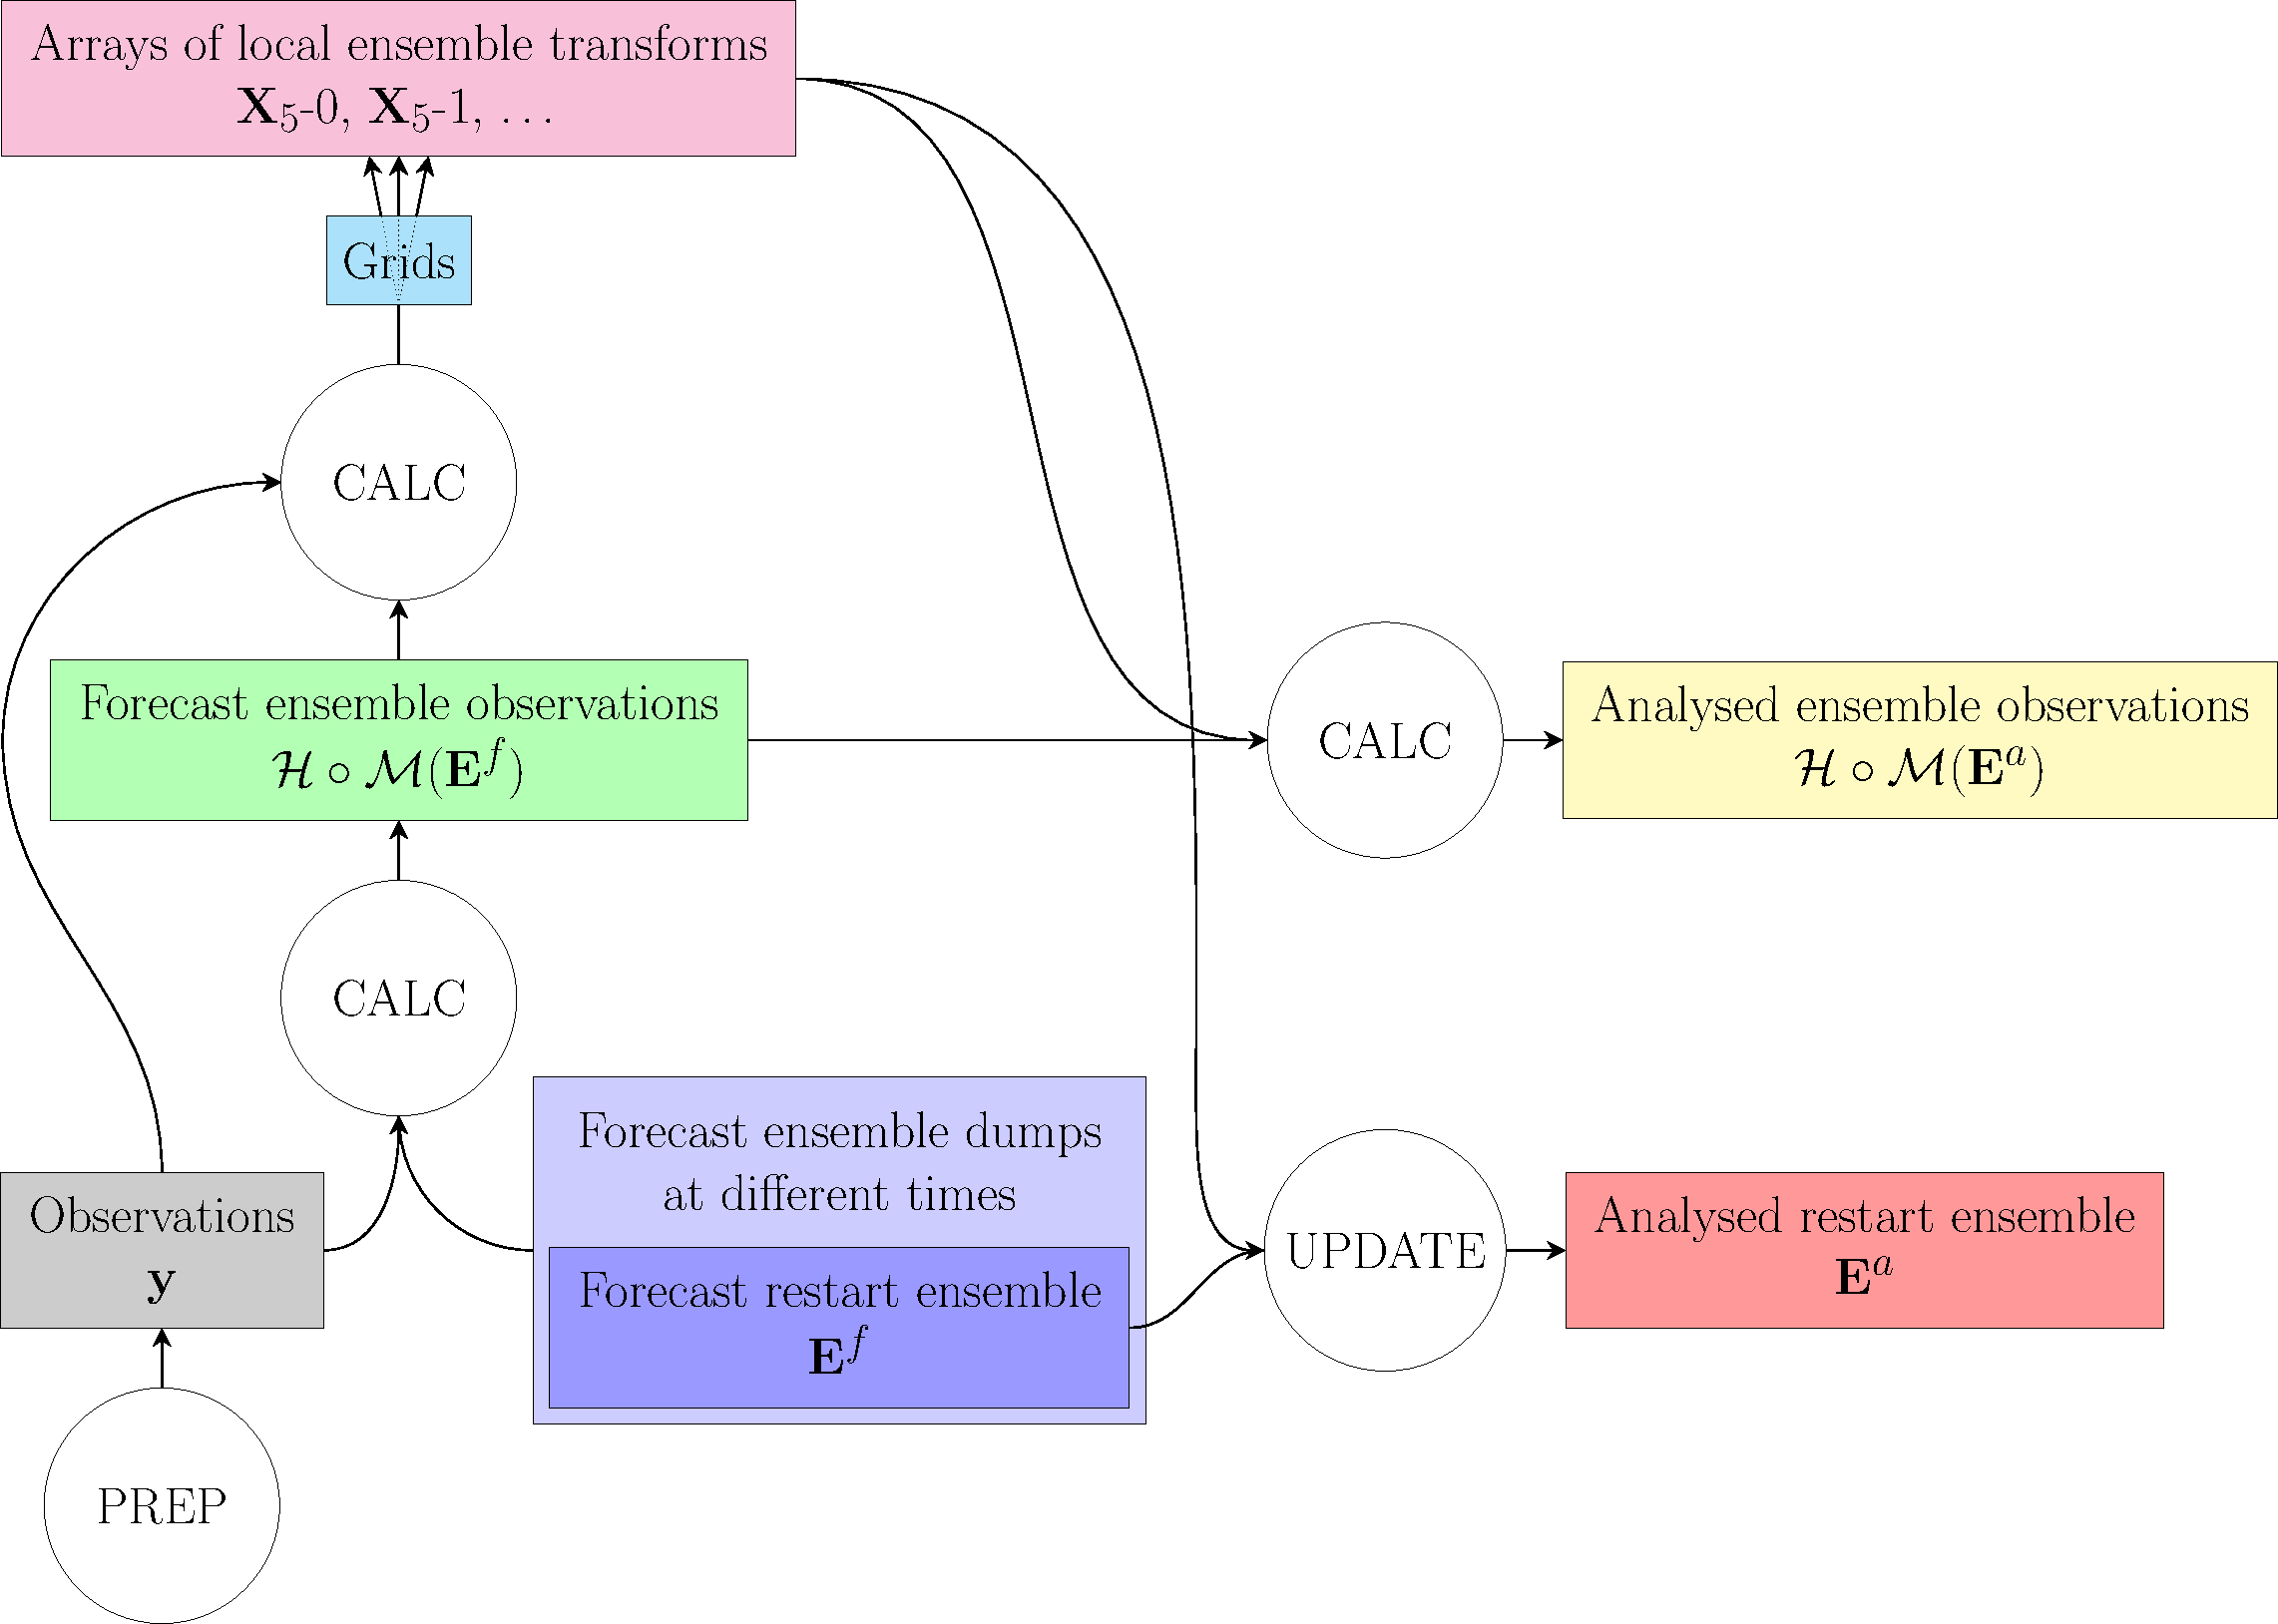
\includegraphics[width = 0.99\textwidth]{plots/enkfc.pdf}
  \caption{The principle diagram of EnKF-C workflow.}
  \label{fig:calcupdate}
\end{figure}

\section{Starting up: example 1}
\label{example1}

It may be a good idea to start getting familiar with the system by running the example in \verb|examples/1|.
The example has been put up based on runs of the regional EnKF and EnOI reanalysis systems for Tasman Sea developed by Bureau of Meteorology. 
It allows one to conduct a single assimilation for 23 December 2007 (day 6565 since 1 January 1990) with either EnKF or EnOI.
To reduce the size of the system, the model state has been stripped down to two vertical levels and $100 \times 100$ horizontal grid.
Due to its size (almost 80\,MB) the data for this example is available for download separately from the EnKF-C code -- see \verb|examples/1/README| for details.

\section{Parameter files}

EnKF-C requires 5 parameter files to run (fig.~\ref{fig:prm}):
\begin{itemize} 
\item main parameter file;
\item model parameter file;
\item grid parameter file;
\item observation types parameter file;
\item and observation data parameter file.
\end{itemize}
Examples of these parameter files can be found in \verb|examples/1|.
Running EnKF-C binaries with \verb|--describe-prm-format| in the command line provides information on the parameter file formats.

\begin{figure}[h]
  \centering
  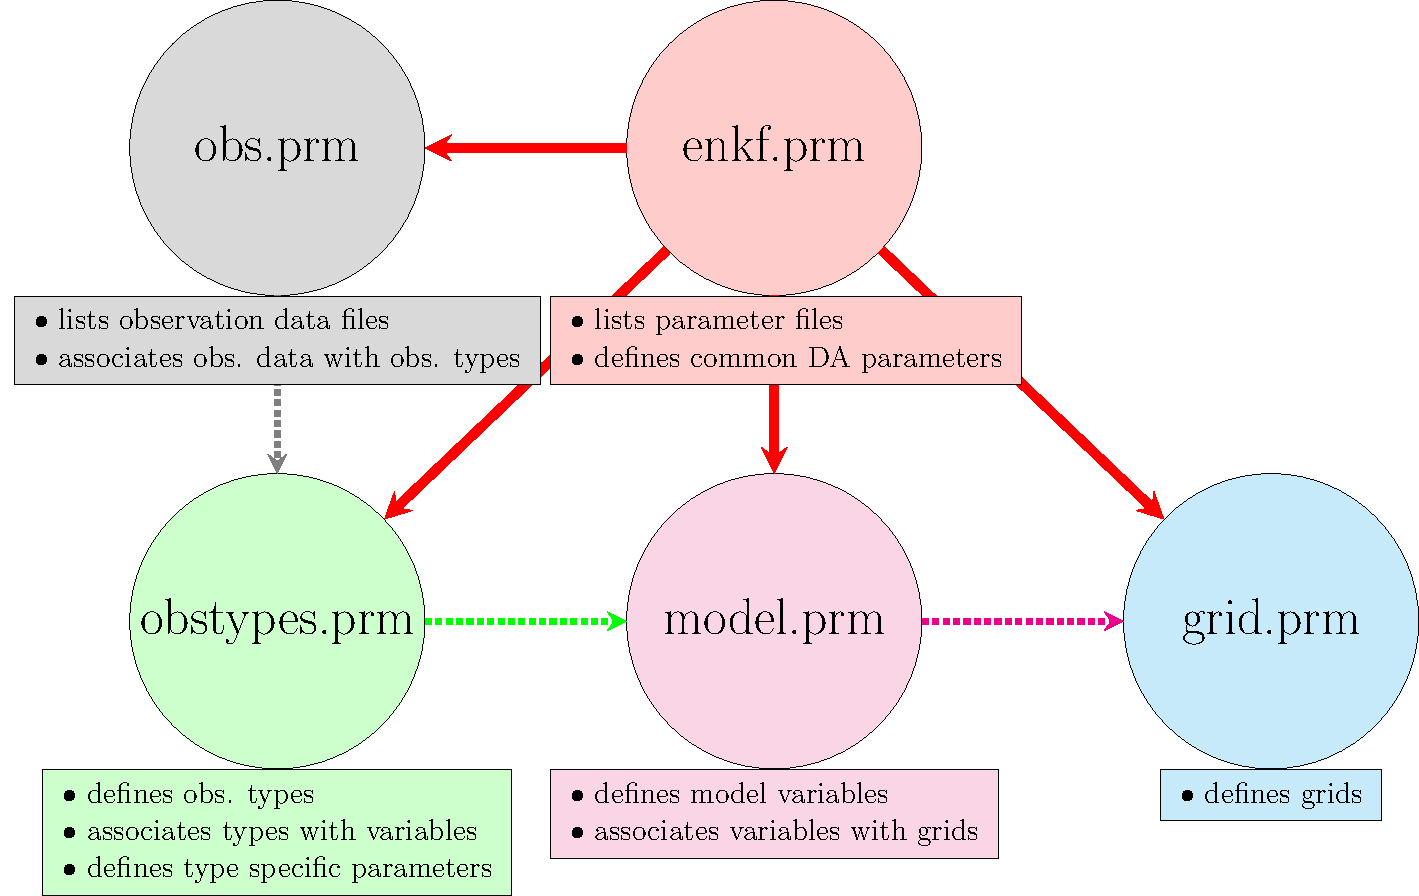
\includegraphics[width=0.8\textwidth]{plots/prm.pdf}
  \caption{Parameter files in EnKF-C.}
  \label{fig:prm}
\end{figure}

\subsection{Main parameter file}
\label{sec:mainprm}

The main parameter file specifies the main parameters of DA and 4 other parameter files.
Its format is described by running \verb|enkf_prep|, \verb|enkf_calc| or \verb|enkf_update| with option \verb|--describe-prm-format|:
\begin{Verbatim}[frame=single,fontsize=\footnotesize]
>./bin/enkf_prep --describe-prm-format

  Main parameter file format:

    MODE            = { ENKF | ENOI }
  [ SCHEME          = { DENKF* | ETKF } ]
  [ ALPHA           = <alpha> ]                              (1*)
    MODEL           = <model prm file>
    GRID            = <grid prm file>
    OBSTYPES        = <obs. types prm file>
    OBS             = <obs. data prm file>
    DATE            = <day of analysis>
  [ WINDOWMIN       = <start of obs window in days from analysis> ] (-inf*)
  [ WINDOWMAX       = <end of obs window in days from analysis> ]   (+inf*)
    ENSDIR          = <ensemble directory>
    BGDIR           = <background directory>                 (MODE = ENOI)
  [ KFACTOR         = <kfactor> ]                            (NaN*)
  [ RFACTOR         = <rfactor> ]                            (1*)
    ...
    LOCRAD          = <loc. radius in km> ...
  [ LOCWEIGHT       = <loc. weight> ... ]                    (# LOCRAD > 1)
  [ NLOBSMAX        = <max. number of local obs. of each type> ]
  [ STRIDE          = <stride for superobing> ]              (1*)
  [ SOBSTRIDE       = <stride for ensemble transforms> ]     (1*)
  [ FIELDBUFFERSIZE = <fieldbuffersize> ]                    (1*)
  [ INFLATION       = <inflation> [ <VALUE>* | PLAIN ]       (0.5*)
    ...
  [ REGION          = <name> <lon1> <lon2> <lat1> <lat2>
    ...
  [ POINTLOG        <lon> <lat> [grid name]]
    ...
  [ EXITACTION      = { BACKTRACE* | SEGFAULT } ]
  [ BADBATCHES      = <obstype> <max. bias> <max. mad> <min # obs.> ]
  [ NCFORMAT        = { CLASSIC | 64BIT | NETCDF4 } ]        (64BIT*)
  [ NCCOMPRESSION   = <compression level>                    (0*) ]
    ...

  Notes:
    1. { ... | ... | ... } denotes the list of possible choices
    2. [ ... ] denotes an optional input
    3. ( ... ) is a note
    4. * denotes the default value
    5. < ... > denotes a description of an entry
    6. ... denotes repeating the previous item an arbitrary number of times
\end{Verbatim}

\subsubsection{Global analysis}

It is possible to conduct global analysis by setting \verb|LOCRAD| and \verb|STRIDE| to large numbers.
This is demonstrated by target ``global'' in example 1.

\subsection{Model parameter file}
\label{sec:modelprm}

The model parameter file mainly describes the composition of the state vector by listing the model variables and specifying the associated grids.

\begin{Verbatim}[frame=single,fontsize=\footnotesize]
>./bin/enkf_prep --describe-prm-format model

  Model parameter file format:

    NAME      = <name>

    VAR       = <name>
  [ GRID      = <name> ]                    (# grids > 1)
  [ INFLATION = <value> [<value> | PLAIN] ]
  [ RANDOMISE <deflation> <sigma> ]

  [ <more of the above blocks> ]
\end{Verbatim}

Each model variable is described in a block started by the entry for the variable name.
The inflation parameters for a variable, if specified, override the common values set in the main parameter file (sec.~\ref{sec:capping}).
Entry RANDOMISE makes it possible to specify a ``forgetting'' model for a variable (sec.~\ref{sec:bias}).

EnKF-C permits using multiple model grids.
In this case each model variable must be associated with one of the grids defined in the grid parameter file.
See \verb|examples/4| for an example.

\subsection{Grid parameter file}
\label{sec:gridprm}

Grid parameter file describes grids used for model variables.
Each grid is described in a section started by the grid name entry and contains the grid name, grid data file, and names of the dimensions and coordinates in the grid data file.
It also contains variable names for the depth and for number of layers in a vertical column (z grids) or land mask (sigma grids):
\begin{Verbatim}[frame=single,fontsize=\footnotesize]
>./bin/enkf_prep --describe-prm-format grid

  Grid parameter file format:

    NAME             = <name> [ PREP | CALC ]
  [ DOMAIN           = <domain name> ]
    VTYPE            = { z | sigma | hybrid }
  [ VDIR             = { fromsurf* | tosurf } ]
  [ MAPTYPE          = { kdtree* | binary } ]             (curvilinear grids)
    DATA             = <data file name>
    XVARNAME         = <X variable name>
    YVARNAME         = <Y variable name>
    ZVARNAME         = <Z variable name>                  (z)
  [ ZCVARNAME        = <ZC variable name> ]               (z)
    CVARNAME         = <Cs_rho variable name>             (sigma)
  [ CCVARNAME        = <Cs_w variable name> ]             (sigma)
  [ SVARNAME         = <s_rho variable name> ]            (uniform*) (sigma)
  [ SCVARNAME        = <s_w variable name> ]              (uniform*) (sigma)
  [ HCVARNAME        = <hc variable name> ]               (0.0*) (sigma)
  [ DEPTHVARNAME     = <depth variable name> ]            (z | sigma)
  [ NUMLEVELSVARNAME = <# of levels variable name> ]      (z)
  [ MASKVARNAME      = <land mask variable name> ]        (sigma | hybrid)
    AVARNAME         = <A variable name>                  (hybrid)
    BVARNAME         = <B variable name>                  (hybrid)
  [ ACVARNAME        = <AC variable name> ]               (hybrid)
  [ BCVARNAME        = <BC variable name> ]               (hybrid)
    P1VARNAME        = <P1 variable name>                 (hybrid)
    P2VARNAME        = <P2 variable name>                 (hybrid)
  [ STRIDE           = <stride for ensemble transforms> ] (1*)
  [ SOBSTRIDE        = <stride for superobing> ]          (1*)
  [ SFACTOR          = <spread factor> ]                  (1.0*)
  [ ZSTATINTS        = [<z1> <z2>] ... ]

  [ <more of the above blocks> ]
\end{Verbatim}

The code is supposed to automatically identify the type of horizontal grid used, while the type of the vertical grid has to be specified explicitly.

\subsubsection{Horizontal grids}
\label{sec:hgrid}

At the moment, EnKF-C supports 3 main types of horizontal grids:
\begin{itemize}
\item equidistant rectangular grids aligned with physical coordinates;
\item non-equidistant rectangular grids aligned with physical coordinates;
\item quadrilateral grids (via libgu).
\end{itemize}
For rectangular grids the code tries to determine and handle periodicity in X direction.

Horizontal grids are parsed either into K-D tree (default from v1.101.4) or into binary tree (default prior to v1.101.4).
Parsing into K-D trees permits use of non-simply connected grids (like tri-polar ORCA grids) and is more memory efficient (see sec.~\ref{sec:memory}).
Note that the code does not detect and therefore can not take advantage of periodic curvilinear grids; because of that, it does not map (skips) observations in cells connecting the grid edges.

Handling non-simply connected grids with parsing into the binary tree requires a bit of effort.
It involves creating an auxiliary grid that is simply connected in grid index space by masking some nodes (replacing their coordinates with NaNs) in the original grid.
Because only PREP requires mapping from physical to grid space, this auxiliary grid is then used in PREP only, while the original grid is used in CALC and UPDATE.
To specify that a grid entry is to be used in PREP only one needs to add qualifier ``PREP'' after its name; and to specify that it is to be used in CALC and UPDATE one needs to add qualifier ``CALC''.
See \verb|examples/3| for an example.

\subsubsection{Vertical grids}

The vertical coordinates are used for mapping the depth/height (pressure) of non-surface observations to fractional layer index.
The observation depth or height are assumed to be positive.

EnKF-C supports 3 types of vertical grids: $Z$; $\sigma$; and hybrid $\sigma$-$p$ ($\sigma$ - pressure).

For $Z$ grids one needs to define vertical coordinates of layer centres (entry \verb|ZVARNAME|) and (optionally) the coordinates of layer corners (\verb|ZCVARNAME|).
If coordinates of layer corners are not specified they are built by the code assuming that the surface layer starts at $z = 0$.

For $\sigma$ grids the code implements the ``new'' vertical coordinate formulation from ROMS as described in \url{https://www.myroms.org/wiki/Vertical_S-coordinate}, Eq.~2 and elaborated by Shchepetkin in \url{https://www.myroms.org/forum/viewtopic.php?f=20&t=2189}.
This formulation reduces to the ``standard'' $\sigma$ grid if the entry \verb|HCVARNAME| is not specified or if the corresponding variable in the grid file is set to zero.
Similarly to $Z$ grid, one needs to define the vertical coordinates of layer centres (entry \verb|CSRVARNAME|) and (optionally) the coordinates of layer corners (entry \verb|CSWVARNAME|).
From version 1.81.0 one can also specify variables for layer coordinates (which is used to be ``plain'' sigma, that is uniform) via entries \verb|SVARNAME| and \verb|SCVARNAME|.

The hybrid $\sigma$-$p$ grids are implemented as described in \url{https://journals.ametsoc.org/doi/pdf/10.1175/2008MWR2537.1}.
One needs to specify the $A$ (\verb|AVARNAME|) and $B$ (\verb|BVARNAME|) arrays for layer centres as well as the top and surface pressure (\verb|P1VARNAME| and \verb|P2VARNAME|).
One can also specify optional $A$ and $B$ arrays for layer corners (\verb|ACVARNAME|, \verb|BCVARNAME|).
The entry \verb|DEPTHVARNAME| needs only to be specified for variables with non-surface observations.

By default, the code assumes that the surface is at layer 0.
If this is not the case, one needs to describe it explicitly by the entry \verb|VDIR = TOSURF|; otherwise the surface ensemble or background observations will not be calculated correctly.

\subsection{Observation types parameter file}
\label{sec:obstypesprm}

Observation types are the interface that connects model and observations.
They are specified in a separate parameter file.
Each observation type is described in a separate section identified by the entry \verb|NAME|.
Apart from the type name, the section must contain the tag for the associated model variable and the tag for the associated observation operator.
The optional parameters include the R-factor and localisation radius for the type (sec.~\ref{sec:datuning}), the allowed range, and spatial limits for the corresponding observations.
\begin{Verbatim}[frame=single,fontsize=\footnotesize]
>./bin/enkf_prep --describe-prm-format obstypes

  Observation types parameter file format:

    NAME        = <name>
  [ DOMAINS     = <domain name> ... ]
    ISSURFACE   = {0 | 1}
  [ STATSONLY   = {0* | 1} ]
    VAR         = <model variable name> ...
  [ ALIAS       = <variable name used in file names> ]   (VAR*)
  [ OFFSET      = <file name> <variable name> ]          (none*)
  [ MLD_VARNAME = <model varname> ]                      (none*)
  [ MLD_THRESH  = <threshold> ]                          (NaN*)
  [ HFUNCTION   = <H function name> ]                    (standard*)
  [ ASYNC       = <time interval> [c*|e [time varname]]] (0*)
  [ LOCRAD      = <loc. radius in km> ... ]
  [ LOCWEIGHT   = <loc. weight> ... ]                    (# LOCRAD > 1)
  [ RFACTOR     = <rfactor> ]                            (1*)
  [ NLOBSMAX    = <max. allowed number of local obs.> ]  (inf*)
  [ ERROR_STD_MIN = <min. allowed superob error> ]       (0*)
  [ SOBSTRIDE   = <stride for superobing> ]              (1*)
  [ MINVALUE    = <minimal allowed value> ]              (-inf*)
  [ MAXVALUE    = <maximal allowed value> ]              (+inf*)
  [ XMIN        = <minimal allowed X coordinate> ]       (-inf*)
  [ XMAX        = <maximal allowed X coordinate> ]       (+inf*)
  [ YMIN        = <minimal allowed Y coordinate> ]       (-inf*)
  [ YMAX        = <maximal allowed Y coordinate> ]       (+inf*)
  [ ZMIN        = <minimal allowed Z coordinate> ]       (-inf*)
  [ ZMAX        = <maximal allowed Z coordinate> ]       (+inf*)
  [ WINDOWMIN   = <start of obs window in days from analysis> ] (-inf*)
  [ WINDOWMAX   = <end of obs window in days from analysis> ]   (+inf*)

  [ <more of the above blocks> ]
\end{Verbatim}

The tags for available observation operators are listed in array \verb|allhentries| in file \verb|calc/allhs.c|.

The \verb|OFFSET| entry may be used for adding the known model bias to observations, for example, to specify the mean dynamic topography (MDT) when assimilating sea level anomaly (SLA) observations.

The localisation radius for an observation type, if specified, overrides the
common value from the main parameter file.
The R-factors for each observation type are obtained by multiplying the common
value by the observation type value.
(More on localisation radius and R-factor in sec.~\ref{sec:datuning}.)

The entries \verb|MLD_VARNAME| and \verb|MLD_THRESH| are used to calculate the model mixed layer depth for projecting the surface bias.

\verb|WINDOWMIN| and \verb|WINDOWMAX| define the allowed temporal interval for this observation type relatively to the analysis day and override the corresponding common settings in the main parameter file.

The use of \verb|ALIAS| is described in sec.~\ref{sec:filenames}.

\subsection{Observation data parameter file}

Observation data parameter file specifies observations to be assimilated.
EnKF-C has a simple policy in this regard: if a data file is listed in the observation data parameter file, then observations from this file are assimilated.
This allows one using custom observation windows for particular observation types, instruments etc., specifying details on the script level during the parameter file generation.

In practice some of observations specified in the observation data parameter file can be outside the observation time window for the cycle.
In this case the exact boundaries of the observation window can be specified by entries \verb|WINDOWMIN| and \verb|WINDOWMAX| in the main parameter file or (for specific observation types) observation types parameter file;
observations with time outside interval \verb|[DATE-WINDOWMIN, DATE+WINDOWMAX)| will be discarded.

The observation parameter file contains an arbitrary number of sections identified by entries \verb|PRODUCT|.
Each section specifies the observation type, input files, reader and, possibly, observation error:
\begin{Verbatim}[frame=single,fontsize=\footnotesize]
./bin/enkf_prep --describe-prm-format obsdata

  Observation data parameter file format:

    PRODUCT   = <product>
    READER    = <reader>
  [ PARAMETER <name> = <value> ]
    ...
    TYPE      = <observation type>
    FILE      = <data file wildcard> 
    ...
  [ ERROR_STD = { <value> | <data file> <varname> } [ EQ* | PL | MU | MI | MA ] ]
    ...

  [ <more of the above blocks> ]
\end{Verbatim}
Observation files can be defined using wildcards ``*'' and ``?''.
Missing a file is reported in the log and is not considered to be a fatal error.

The line in the above example starting with \verb|ERROR_STD| specifies the observation error.
It can contain either a number or a file name.
In the case of entering the file name there also should be another entry in the same line specifying the name of the variable to be read.
The variable should have the same dimension (2D or 3D) as the associated observation kind as described by the field \verb|issurface| in the array \verb|allkinds| in file \verb|common/obstypes.c| (sec.~\ref{sec:obstypesprm}).

The line with observation error can also have another token specifying the type of operation to be conducted: \verb|EQUAL| ($\sigma_{tot} \leftarrow \sigma_{now}$, default), \verb|PLUS| ($\sigma_{tot} \leftarrow \sqrt{\sigma_{tot}^2 + \sigma_{now}^2}$), \verb|MULT| ($\sigma_{tot} \leftarrow \sigma_{tot} \sigma_{now}$), \verb|MIN| ($\sigma_{tot} = \max(\sigma_{tot}, \sigma_{now})$), or \verb|MAX| ($\sigma_{tot} = \min(\sigma_{tot}, \sigma_{now})$).
There can be several error entries in a section in the observation parameter file.

The observation time only matters if the observation type is specified to be ``asynchronous'' (see sec. \ref{sec:async}).
In this case the model estimation for the observation is made by using model state at the appropriate time.
Otherwise, observations are assumed to be made at the time of assimilation, regardless of the actual observation time.

Note that there can be multiple blocks with the same product.
This enables custom treatment of some specific data.
For example, the following entries override observation error for Geosat (files with prefix \verb|g1_|) on 23 May 2006:
\begin{Verbatim}[frame=single,fontsize=\footnotesize]
# set observation error for Geosat to 7cm
product == RADS
type = SLA
reader = standard2
file=/short/p93/pxs599/obs/RADS-IB/y2006/m05/g?_d23.nc
error_std = 0.07

# use default errors for other altimeters
product == RADS
type = SLA
reader = standard2
file=/short/p93/pxs599/obs/RADS-IB/y2006/m05/[!g]?_d23.nc
\end{Verbatim}

\section{File name conventions}
\label{sec:filenames}

EnKF-C assumes that the ensemble and background file names have some predefined formats.
The file name for member \verb|mid| and model variable \verb|varname| is assumed to be \spverb|sprintf("mem%03d_%s.nc", mid, varname)|.
The background file (EnOI only) for variable \verb|varname| is assumed to be \spverb|sprintf("bg_%s.nc", varname)|.
The above names are used for reading forecast states for synchronous DA and for writing analyses, in the case if the analyses are appended to forecasts (true by default).
For asynchronous DA the member and background file names for the time slot \verb|t| are assumed to be \spverb|sprintf("mem%03d_%s_%d.nc", mid, varname, t)| and \spverb|sprintf("bg_%s_%d.nc", varname, t)|, correspondingly.

There are possible situations when the surface field and 3D field of the same variable have different asynchronous settings.
For example, the sea surface temperature (SST) may have asynchronous time intervals of 0.25 days, while for the subsurface temperature these may be set to 1 day.
In such cases there is a clash between the corresponding asynchronous file names.
To resolve it, one (or both) fields should use an alias instead of the model variable name in its file name specified by the entry ALIAS of the corresponding observation type.

\section{PREP}

PREP is the first stage of data assimilation in EnKF-C.
Its preprocesses observations by bringing them to a common form and merging close observations into so called superobservations.

By design, PREP is supposed to be light-weight, so that it does not read either the ensemble or background, and the only model information it needs is the model grid. 
(Note that this may require some additional processing at later stages for models with dynamic grid, such as HYCOM.)

The name of the binary (executable) for PREP is \verb|enkf_prep|.
It has the following usage and options:
\begin{Verbatim}[frame=single,fontsize=\footnotesize]
>./bin/enkf_prep
  Usage: enkf_prep <prm file> [<options>]
  Options:
  --consider-subgrid-variability
      increase error of superobservations according to subgrid variability
  --describe-prm-format [main|model|grid|obstypes|obsdata]
      describe format of a parameter file and exit
  --describe-superob <sob #>
      print composition of this superobservation and exit
  --log-all-obs
      write all obs to observations-orig.nc (default: obs within model domain only)
  --no-superobing
  --no-superobing-across-instruments
  --no-thinning
  --no-writing-orig-obs
  --version
      print version and exit
\end{Verbatim}

\verb|enkf_prep| writes the preprocessed observations to file \verb|observatons.nc|.
It also writes original (not superobed) observations to \verb|observatons-orig.nc| (provided that superobing has not been switched off by flag \verb|--no-superobing|).
By default, only observations within the model grid are written to it, but the the option \verb|--log-all-obs| changes this behaviour to writing all observations from the input files.

\subsection{Observation types, products, instruments, batches, readers}

\subsubsection{Types}
\label{sec:types}

Each observation has a number of attributes defined by the fields of the structure \verb|observation|.
One of them is observation type, which characterises the observation in a general way and relates it to the model state.
For example, typical oceanographic observations may have tags SLA (for sea level anomalies), SST (sea surface temperature), TEM (subsurface temperature) and SAL (subsurface salinity).
Different types can be related to the same model variable, as do SST and TEM in the above example.
Observation types are described in the corresponding parameter file (sec.~\ref{sec:obstypesprm}).

\subsubsection{Products}

An observation is also characterised by ``product''.
It can be a tag for an organisation that provides data from certain observational platforms, e.g.:
\begin{Verbatim}[frame=single,fontsize=\footnotesize]
PRODUCT == RADS
TYPE = SLA
READER = standard2
FILE = obs/RADS-IB/y2007/m12/??_d19.nc
FILE = obs/RADS-IB/y2007/m12/??_d20.nc
FILE = obs/RADS-IB/y2007/m12/??_d21.nc
FILE = obs/RADS-IB/y2007/m12/??_d22.nc
FILE = obs/RADS-IB/y2007/m12/??_d23.nc

PRODUCT == NAVO
TYPE = SST
READER = standard
FILE = obs/NAVO/navo_20071219.nc
FILE = obs/NAVO/navo_20071220.nc
FILE = obs/NAVO/navo_20071221.nc
FILE = obs/NAVO/navo_20071222.nc
FILE = obs/NAVO/navo_20071223.nc
\end{Verbatim}

\subsubsection{Instruments}

The observational data from a product can be collected by a number of instruments.
The corresponding field in the \verb|measurement| structure is supposed to be filled by the observation reader.

\subsubsection{Batches}

An observation can be attributed to one of the groups called ``batches'', such as altimeter passes, Argo profiles etc., to enable detection and discarding of bad batches.
Programmatically, to switch on capabilities associated with observation batches for a particular kind of observations, the observation batch ID needs to be set by the corresponding observation reader.

A batch of observations is considered bad if either its mean innovation or mean absolute innovation exceed specified thresholds.
Specifications for bad batches can be set in the parameter file as follows:
\begin{Verbatim}[frame=single,fontsize=\footnotesize]
BADBATCHES = SLA 0.06 0.10 500
BADBATCHES = TEM 4 5 0
BADBATCHES = SST 0.3 0.5 10000
BADBATCHES = SAL 1.5 2 0
\end{Verbatim}
The above entry means that any batch of observations of type SLA (typically, an orbit) containing more than 500 observations and having either mean innovation greater than 0.06 (meter) in magnitude or mean absolute innovation greater than 0.10 is considered to be bad.
Similarly, a TEM batch (typically, a profile) is considered bad if the mean innovation exceeds 4 (degrees) or the mean absolute innovation exceeds 5 (degrees).
The parameter file can have an arbitrary number of such entries.
Information about bad batches is written by \verb|enkf_calc| to the file \verb|badbatches.out|.
When \verb|enkf_prep| detects the presence of such file, it marks the corresponding observations as bad.

Therefore, the workflow for detecting and eliminating bad batches of observations is as follows:
\begin{enumerate}
\item specify bad batches in the parameter file;
\item make a pilot run of \verb|enkf_prep|;
\item run \verb|enkf_calc| with the flag \verb|--forecast-stats-only|;
\item remove \verb|observations.nc| and \verb|observations-orig.nc|;
\item calculate analysis in a ``normal'' way by running \verb|enkf_prep|, \verb|enkf_calc| and \verb|enkf_update|.
\end{enumerate}

Note that bad batches are identified by CALC based on superobservations formed by observations from the same batch only.
Consequently, detection of bad batches may become unreliable if there are not enough such ``clean'' superobservations.
It is possible to alleviate this problem by (1) switching off superobing by the option \verb|--no-superobing| for \verb|enkf_prep| or (2) as a compromise, by running \verb|enkf_prep| with \verb|--no-superobing-across-instruments|.

\subsubsection{Readers}

The function of data readers is to read observations in specified files and parse them sequentially into \verb|struct observation| defined in \verb|common/observations.h|.

At the moment there are few agreed standards for observational data.
Even data of similar kind may have specific features that require creating a new or modify an existing observation data reader.
It is therefore likely that developing a completely new system will require add new data readers.

The new readers can be created based on existing ones, or developed from scratch.
The available readers are listed by the variable \verb|allreaders| defined in \verb|prep/allreaders.c|.
Each reader can be specified in the observation data parameter file with an arbitrary number of parameters.
For example, the following section changes the default minimal depth for using altimetry observations to 150\,m:
\begin{Verbatim}
(...)
product == RADS
type = SLA
reader = standard2
parameter MINDEPTH = 150
(...)
\end{Verbatim}

There are also several generic readers:
\begin{Verbatim}
reader_xy_scattered
reader_xy_gridded
reader_xyz_scattered
reader_xyz_gridded
reader_xyh_gridded
\end{Verbatim}
These readers allow one to specify a number of parameters by means of the entry \verb|PARAMETER| of the observation data parameter file.
One obligatory parameter for these readers is \verb|VARNAME|; a number of other obligatory parameters (e.g. \verb|LONNAME|, \verb|LATNAME|) can be specified either via the entry \verb|PARAMETER| or by using default variable names in data files.

\subsection{Superobing}

``Superobing'' is the process of reduction of the number of observations by merging spatially close observations before their assimilation.
EnKF-C merges observations if:
\begin{itemize}
\item they belong to the same model grid cell;
\item are of the same type;
\item for asynchronous observations -- belong to the same time slot.
\end{itemize}
The horizontal size of superobing cells can be increased from the default of 1 model grid cell to $N \times N$ cells by setting \verb|SOBSTRIDE = <N>| in the parameter file; the vertical size is always equal to 1 layer.
Setting \verb|SOBSTRIDE = 0| switches superobing off.

The observations are merged by averaging their values, coordinates and times with weights inversely proportional to the observation error variance.
The observation error variance of a superobservation is set to the inverse of the sum of inverse observation error variances of the merged observations.
The product and instrument fields of the superobservation are set either to those of the merged observations or to -1, depending on whether the merged observations have the same values for these fields or not.

Command line parameter \verb|--consider-subgrid-variability| switches on considering the subgrid variability by calculating standard deviation of the merged observations $\sigma\!_{sub}$ and using $\sigma\!_{obs} = \max(\sigma\!_{obs}, \sigma\!_{sub})$.
The calculation of $\sigma\!_{sub}$ is currently done in a rather crude way, assuming equal weights for all merged observations.

Note that during superobing EnKF-C by default thins observations with identical positions, assuming that those must been obtained from high-frequency instruments (e.g. moorings).
This thinning can be switched off by the command line parameter \verb|--no-thinning|.

\subsection{Asynchronous DA / FGAT}
\label{sec:async}

An observation type can be specified as ``asynchronous'' by specifying entry \verb|ASYNC| in the observation types parameter file (sec. \ref{sec:obstypesprm}), e.g.:
\begin{Verbatim}[frame=single,fontsize=\footnotesize]
NAME = SST
(...)
ASYNC = 1
(...)
\end{Verbatim}
The above means that SST observations are considered to be asynchronous with time bins of 1 day.
If, for example, the assimilation time is specified as ``6085.5 days since 1990-01-01'', then the interval 0 is centred (by default) at the time of assimilation, i.e. will be from day 6080.0 to day 6081.0; interval -1 -- from day 6079.0 to day 6080.0, interval 1 -- from day 6081.0 to day 6082.0, and so on.
It is possible to shift the asynchronous intervals so that not the centre but the start of interval 0 is located at the time of assimilation.
In this case one needs to add qualifier ``e'' after the length of the interval, i.e.
\begin{Verbatim}[frame=single,fontsize=\footnotesize]
NAME = SST
(...)
ASYNC = 1 e
(...)
\end{Verbatim}
The interval 0 will then be from day 6085.5 to day 6086.5.

The model dumps for each asynchronous interval are read from files with names \spverb|mem<xxx>_<variable name>_<time shift>.nc| in the ensemble directory (for the EnKF) or \spverb|bg_<variable name>_<time shift>.nc| in the background directory (for the EnOI).
Here ``time shift'' is the interval ID (with the interval 0 being centred/starting at the observation time).
If the corresponding members (or the background files, in the case of EnOI) are found, the observations are assimilated asynchronously; if they are not found, then the observations are assimilated synchronously.
This can be tracked from the CALC log file, e.g.:
\begin{Verbatim}[frame=single,fontsize=\footnotesize]
  calculating ensemble observations:
  2014-03-22 06:28:28
    ensemble size = 96
    distributing iterations:
      all processes get 6 iterations
      process 0: 0 - 5
    SST |aaaaaa|aaaaaa|aaaaaa|aaaaaa|aaaaaa
    SLA |aaaaaa|aaaaaa|aaaaaa|aaaaaa|aaaaaa
    TEM ......
    SAL ......
\end{Verbatim}
The entries ``a'' mean that the observations are assimilated asynchronously and the files and the corresponding (by name) files have been found.
These entries would be replaced by ``s'' if the observations were assimilated synchronously because of lacking the corresponding files.
The vertical lines indicate the time slots for asynchronous DA; in the above example the DAW has 5 time slots.
The entries ``.'' indicate calculating ensemble observations for synchronous observations.
Note that only the master process is writing to the log here, which explains why there is only output from 6 members in the log above.

Fig.~\ref{fig:mom_timing} shows an example of observation timing in a MOM based ocean forecasting system with a 3-day assimilation cycle.
In this system the ``fast'' SST data is assimilated asynchronously with 6\,h intervals using model fields averaged over these intervals; the slower SLA data is assimilated asynchronously with 24\,h intervals using daily model dumps; and in-situ T and S fields are assimilated synchronously.
This is achieved with the following settings in the observation types parameter file:
\begin{Verbatim}[frame=single,fontsize=\footnotesize]
NAME = SLA
VAR = eta_t
ISSURFACE = yes
ASYNCHRONOUS 1
<...>
NAME = SST
VAR = temp sstb
ISSURFACE = yes
ASYNCHRONOUS 0.25 E
<...>
NAME = TEM
VAR = temp sstb
ISSURFACE = no
<...>
NAME = SAL
VAR = salt
ISSURFACE = no
<...>
\end{Verbatim}
\begin{figure}[h]
  \centering
  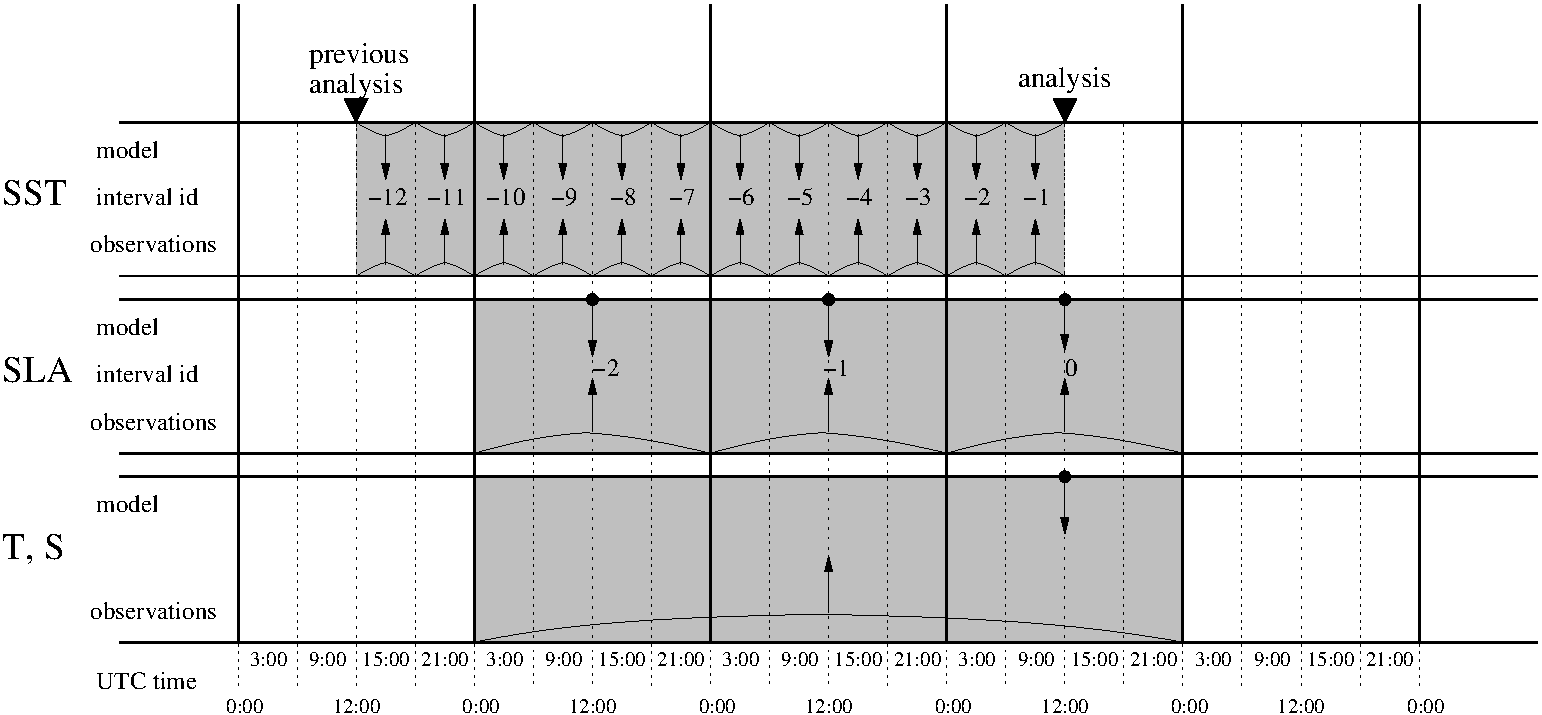
\includegraphics[width = \textwidth]{plots/obstiming_example.pdf}
  \caption{Example of observation timing in a MOM based ocean forecasting system.}
  \label{fig:mom_timing}
\end{figure}

From version 1.101.0 the code can check whether the time of the model dump used to calculate forecast observations matches the time of the (centre of the) corresponding observation window.
To activate this check, one needs to add the name of the time variable in the model dump after the timing qualifier ``c'' or ``e''.
For the example above the first two sections of the observation types parameter file would the look as follows:
\begin{Verbatim}[frame=single,fontsize=\footnotesize]
NAME = SLA
VAR = eta_t
ISSURFACE = yes
ASYNCHRONOUS 1 C Time
<...>
NAME = SST
VAR = temp sstb
ISSURFACE = yes
ASYNCHRONOUS 0.25 E Time
<...>
\end{Verbatim}

\section{CALC}

CALC is the second stage of data assimilation in EnKF-C.
It calculates 2D arrays of local ensemble transforms $\mb X_5$ (for EnKF) or coefficients $\mb w$ (for EnOI).

The name of the binary for CALC is \verb|enkf_calc|.
It has the following usage and options:
\begin{Verbatim}[frame=single,fontsize=\footnotesize]
>./bin/enkf_calc 
  Usage: enkf_calc <prm file> [<options>]
  Options:
  --describe-prm-format [main|model|grid|obstypes]
      describe format of a parameter file and exit
  --forecast-stats-only
      calculate and print forecast observation stats only
  --ignore-no-obs
      proceed even if there are no observations
  --no-mean-update
      update ensemble anomalies only
  --point-logs-only
      skip calculating transforms for the whole grid and observation stats
  --print-batch-stats
       calculate and print global biases for each batch of observations
  --single-observation-xyz <lon> <lat> <depth> <type> <inn> <std>
      assimilate single observation with these parameters
  --single-observation-ijk <fi> <fj> <fk> <type> <inn> <std>
      assimilate single observation with these parameters
  --use-rmsd-for-obsstats
      use RMSD instead of MAD when printing observation stats
  --use-these-obs <obs file>
      assimilate observations from this file; the file format must be compatible
      with that of observations.nc produced by `enkf_prep'
  --version
      print version and exit
\end{Verbatim}

The option \verb|--forecast-stats-only| can be used for quick calculation of the innovation statistics for a given background (or ensemble).
This can be used, for example, for obtaining the persistence statistics, that is, the innovation statistics for the previous analysis.

The options \verb|--single-observation-xyz| and \verb|--single-observation-ijk| provide an easy way to conduct the so called single observation experiments, with the observation coordinates provided either in spatial or grid coordinates, correspondingly.
Parameter \verb|<value>| defines innovation rather than the observation value.
Normally, this experiments would be conducted in the EnOI mode, calculating increment (option \verb|--output-increment| of \verb|enkf_update|) rather than analysis.
When run in the EnKF mode, the increment (or analysis, depending on specifications) for each member is calculated.

Note that the calculated transforms \emph{do not} incorporate inflation.
Inflation is applied during UPDATE according to specifications (sec.~\ref{sec:capping}).

\subsection{Observation functions}
\label{sec:hfunctions}

Model estimations for observations of each type are calculated using observation functions specified for this type by entry \verb|HFUNCTIONS| in the observation types parameter file, e.g.:
\begin{Verbatim}[frame=single,fontsize=\footnotesize]
NAME = SLA
...
HFUNCTION = standard
...
\end{Verbatim}
The available functions for each observation type are specified by the variable \verb|allhentries| in \verb|calc/allhs.c|.
The ``standard'' functions do normally perform 2D or 3D linear interpolation from the corner model grid nodes for the cell containing the observation.

\subsection{Interpolation of ensemble transforms}

Local ensemble transforms $\mb X_5$ (EnKF) or local ensemble weights $\mb w$ (EnOI) represent smooth fields with the characteristic spatial variability scale of the localisation radius.
This smoothness allows one to reduce the computational load in CALC by calculating local transforms or weights on a subgrid with a specified stride only, and using linearly interpolated transforms or weights in the intermediate grid cells \citep{yan09a}.
The value of the stride is defined by the \verb|STRIDE| entry in the main parameter file and can be overwritten for a particular grid in the grid parameter file.

\subsection{Adaptive moderation of observations}

One of the standard quality control (QC) procedures in DA is the so called background check, when an observation is compared with the forecast and discarded if the innovation magnitude exceeds some specified threshold.
The downside of this approach is that it can not distinguish between situations of an outlier, big model error (e.g. because of an error in forcing), or model divergence.
While one probably would like to discard an outlier, it is usually desirable to make use of valid observations, although, perhaps, with a reduced impact, to avoid ``over-stressing'' the model.
In EnKF-C this is achieved by adaptive moderation of the observation impact by restricting the magnitude of the increment from a given observation in observation space by $K$ times magnitude of the spread of the forecast ensemble \citep{sak17a}.

Specifically, the adaptive moderation of the observation impact is conducted by smoothly increasing the observation error depending on the magnitude of innovation as follows:
\begin{align*}
  \sigma^2_{obs} \leftarrow \left[(\sigma_{f}^2 + \sigma_{obs}^2)^2 + \sigma_f^2 \, d^2 / K^2\right]^{1/2} - \sigma_f^2,
\end{align*}
where $\sigma_{obs}$ is the observation error standard deviation, $\sigma_f$ -- forecast ensemble spread, $d$ -- innovation, and $K$ -- the so called K-factor defined in the main parameter file (sec. \ref{sec:mainprm}).
Tests with small models show that setting the $K \ge 2$ makes a marginal impact (if any) on performance of weakly suboptimal systems, while still can be quite beneficial in stressful situations.

\subsection{Moderation of spread reduction}

The moderating parameter $\alpha \in (0, 1]$ specified in the main parameter file via the entry \verb|ALPHA| allows one to reduce the contraction of ensemble during assimilation, while leaving the increment unchanged (``relaxation to prior spread'', \citealt{zha04a}, eq.~5).
It modifies the right multiplied ensemble transform matrix as
\begin{align*}
  \mb T_R \leftarrow \mb I + \alpha (\mb T_R - \mb I).
\end{align*}
Setting $\alpha = 0$ results in no update of the ensemble anomalies, while $\alpha = 1$ results in full update.

\subsection{Innovation statistics}

In its course CALC calculates some basic innovation statistics: number of observations, mean absolute forecast innovation, mean absolute analysis innovation, mean forecast innovation, mean analysis innovation, mean forecast ensemble spread, and mean analysis ensemble spread.
This statistics is provided for each region defined in the main parameter file (sec.~\ref{sec:mainprm}), as well as for each time slot defined for asynchronous DA, and for each instrument.
By default, EnKF-C defines one statistical region ``Global'' with domain $[x_1,x_2] = [-999,999], [y_1,y_2] = [-999,999]$.

In addition, for 3D observations CALC also calculates observation statistics in specified depth intervals.
These intervals can be set via the entry \verb|ZSTATINTS| in the grid parameter file; by default, three intervals are defined: \verb|[0 DEPTH_SHALLOW]|, \verb|[DEPTH_SHALLOW DEPTH_DEEP]|, and \verb|[DEPTH_DEEP DEPTH_MAX]|, where \verb|DEPTH_SHALLOW|, \verb|DEPTH_DEEP| and \verb|DEPTH_MAX| are the macros defined in \verb|common/definitions.h|.

Following is an example of innovation statistics written to the log (standard output) of \verb|enkf_calc|:
\begin{Verbatim}[frame=single,fontsize=\footnotesize]
  printing observation statistics:
    region obs.type   # obs.  |for.inn.| |an.inn.|   for.inn.   an.inn.  for.spread  an.spread
    ------------------------------------------------------------------------------------------
    Tasman
           SLA          3003    0.067      0.038      0.033      0.012      0.035      0.025  
            -4           712    0.058      0.038      0.035      0.013      0.028      0.021  
            -3           785    0.093      0.040      0.060      0.019      0.052      0.034  
            -2           700    0.062      0.043      0.030      0.016      0.027      0.021  
            -1           668    0.049      0.031      0.017      0.004      0.028      0.021  
             0           138    0.078      0.033     -0.043     -0.016      0.045      0.029  
             j1         1323    0.070      0.033      0.041      0.016      0.037      0.024  
             n1          876    0.073      0.042      0.052      0.025      0.036      0.026  
             g1          785    0.054      0.042     -0.004     -0.009      0.029      0.024  
             N/A          19    0.101      0.037      0.097      0.031      0.059      0.036  
           SST          9316    0.346      0.174     -0.215     -0.094      0.358      0.254  
            -4          2946    0.327      0.166     -0.236     -0.092      0.342      0.245  
            -3          2733    0.368      0.183     -0.270     -0.133      0.362      0.256  
            -2          2560    0.352      0.169     -0.167     -0.057      0.370      0.262  
            -1           580    0.342      0.191     -0.148     -0.093      0.414      0.291  
             0           497    0.305      0.182     -0.126     -0.075      0.307      0.225  
             AVHRR      9316    0.346      0.174     -0.215     -0.094      0.358      0.254  
           TEM           768    0.581      0.365     -0.245     -0.151      0.320      0.251  
             ARGO        768    0.581      0.365     -0.245     -0.151      0.320      0.251  
             0-50m       125    0.418      0.230      0.049      0.027      0.365      0.281  
             50-500m     451    0.678      0.403     -0.266     -0.141      0.360      0.278  
             >500m       192    0.458      0.365     -0.387     -0.291      0.196      0.170  
           SAL           768    0.079      0.060      0.014      0.019      0.033      0.028  
             ARGO        768    0.079      0.060      0.014      0.019      0.033      0.028  
             0-50m       125    0.079      0.063      0.031      0.035      0.034      0.030  
             50-500m     451    0.092      0.067      0.026      0.032      0.039      0.032  
             >500m       192    0.048      0.041     -0.027     -0.021      0.018      0.016  
\end{Verbatim}
This excerpt shows innovation statistics for the region ``Tasman''.
It contains sections for SST, SLA and TEM observations.
The summary statistics for each observation type is shown at the top of each section; then statistics for days -4, -3, -2, -1 and 0 of a 5-day DAW are shown for the two asynchronous types, SST and SLA.
(More generally, the numbering of time intervals corresponds to their positions relative to the analysis time.
For more details see sec.~\ref{sec:async}.)
After that, statistics for particular instruments is shown; ``N/A'' corresponds to superobservations resulted from merging observations from two or more instruments.
(One can avoid superobing across different instruments by using option \verb|--no-superobing-across-instruments| in \verb|enkf_prep|.)
For subsurface temperature also statistics for shallow (0--50\,m), deep ($>$500\,m), and intermediate (50--500\,m) observations is given.

The analysis innovation statistics is calculated from the updated (analysis) ensemble observations by CALC, thus avoiding the need to access analysis files produced later by UPDATE.
The update of ensemble observations is performed in the same way as that of any other element of the state vector:
for the EnKF -- by applying the appropriate local ensemble transforms to the forecast ensemble observations,
\begin{align*}
  \mathcal H (\mb E^a) \leftarrow \mathcal H (\mb E^f) \, \mb X_5;
\end{align*}
and for the EnOI -- by applying the appropriate local linear combination of the ensemble observation anomalies:
\begin{align*}
  \mathcal H (\mb E^a) \leftarrow \left[ \mathcal H (\mb x^f) + (\mb H \mb A^f) \mb w\right] \mb 1\T + \mb H \mb A^f.
\end{align*}

\subsection{Impact of observations}
\label{sec:impact}

In the course of its work CALC routinely calculates two metrics for assessing the impact of observations, degrees of freedom of signal (DFS) and spread reduction factor (SRF):
\begin{align*}
  & \mathrm{DFS} = \mathrm{tr}(\mb K \mb H) = \mathrm{tr}(\mb G \mb S), \\
  & \mathrm{SRF} = \sqrt{\frac{\mathrm{tr}(\mb H \mb P^f \mb H\T \mb R^{-1})}{\mathrm{tr}(\mb H \mb P^a \mb H\T \mb R^{-1})}} - 1 = \sqrt{\frac{\mathrm{tr}(\mb S\T \mb S)}{\mathrm{tr}(\mb G \mb S)}} - 1,
\end{align*}
where $\mathrm{tr}(\cdot)$ is the trace function.
The values of these metrics for each local analysis, calculated both for all observations and for observations of each type only, are written to file \verb|enkf_diagn.nc|.
Note that the in EnKF-C DFS and SRF are calculated from the above expressions and represent theoretical values for the EnKF analysis; they coincide with the actual DFS and SRF values only for the ETKF, but not for the DEnKF, which is an approximation of the KF (and indeed not for the EnOI, which is not even an approximation).

In the EnKF context DFS is a useful indicator of potential rank problems.
Normally, it should not exceed a fraction (a half, or better, a quarter) of the ensemble size per the characteristic time of the error growth.
SRF shows the ``strength'' of DA.
``Strong'' DA implies a close to optimal system, which indeed never happens in practice.
Therefore, ideally, SRF should be small (below 1, on average).

\subsection{Multiple model grids}

EnKF-C permits using multiple model grids, in which case the ensemble transforms are calculated sequentially for each of the grids.
These transforms are then used for updating the model variables defined on the corresponding grids.

\subsection{Domains}
\label{sec:domains}

By default, all local observations for a given grid node contribute to the corresponding ensemble transform.
Sometimes it is desirable to disconnect observations of certain type from contributing to transforms on particular grids.
For example, it may be desirable in climate systems to disregard observations of the sea surface height in updating the atmospheric variables.
The concept of ``domains'' introduced in v1.89.0 provides a mechanism for handling such situations within a single analysis.
It works as follows.
Each grid can be associated with a certain domain via the optional entry \verb|DOMAIN| in the grid parameter file.
For example, in a climate model one can have domains ``Ocean'' and ``Atmosphere''.
Then entry \verb|DOMAINS| in the observation types parameter file can list domains observations of this type are visible from.
By default, observations of any type are visible from all grids.

\subsection {``Multi-scale'' localisation}

It is possible to specify the localisation taper function as a linear combination of the Gaspari and Cohn's taper functions with different support radii:
\begin{align*}
  f(r) = \sum_{i=1}^N w_i f_0(\frac{r}{R_i}),
\end{align*}
where $w_i$ is the weight, $r$ is the distance, $R_i$ is the support radius, and
\begin{align*}
  f_0(\frac{x}{2}) = \left\{
  \begin{array}{ll}
    1 - \frac{5}{3} x^2 + \frac{5}{8} x^3 + \frac{1}{2} x^4 -\frac{1}{4} x^5, \quad & 0 \le x \le 1,\\
    -\frac{2}{3} x^{-1} + 4 - 5x + \frac{5}{3}x^2 + \frac{5}{8}x^3 - \frac{1}{2} x^4 + \frac{1}{12}x^5, \quad & 1 < x \le 2,\\
    0, \quad & 2 < x.
  \end{array}
  \right.
\end{align*}
This can be set by entries \verb|LOCRAD| and \verb|LOCWEIGHT| either in the main parameter file or in the observation types parameter file, e.g.:
\begin{Verbatim}
  LOCRAD 150 500
  LOCWEIGHT 0.9 0.1
\end{Verbatim}
(recall that entries in the observation types parameter file for particular observation types override the common settings in the main parameter file).
Note that the weights are normalised so that their sum is equal to 1.

\section{UPDATE}

UPDATE is the third and final stage of data assimilation in EnKF-C.
It updates the ensemble (EnKF) or the background (EnOI) by applying the transforms calculated by CALC.

The name of the binary for UPDATE is \verb|enkf_update|.
It has the following usage and options:
\begin{Verbatim}[frame=single,fontsize=\footnotesize]
>./bin/enkf_update
  Usage: enkf_update <prm file> [<options>]
  Options:
  --calculate-spread
      calculate ensemble spread and write to spread.nc
  --calculate-forecast-spread
      calculate forecast ensemble spread only and write to spread.nc
  --describe-prm-format [main|model|grid]
      describe format of a parameter file and exit
  --calculate-vertical-correlations
      calculate correlation coefficients between surface and other layers of
      3D variables and write to vcorr.nc
  --direct-write
      write fields directly to the output file (default: write to tiles first)
  --joint-output
      append analyses to forecast files (default: write to separate files)
  --leave-tiles
      do not delete tiles
  --no-fields-write
      do not write analysis fields
  --output-increment
      output analysis increment (default: output analysis)
  --write-inflation
      write adaptive inflation magnitudes to inflation.nc
  --version
      print version and exit
\end{Verbatim}

The option \verb|--joint-output| tells UPDATE to append analyses to the corresponding forecast files, using new variable names constructed by concatenating the forecast variable names and suffix \verb|_an|.
By default the analyses are written to separate files, using the same variable names as the forecast files, but with an extra suffix \verb|.analysis| or \verb|.increment| added to the file name, depending on whether the analysis or increment is written.

By default, UPDATE first writes each updated horizontal field of the model to a separate file (referred to here as a tile), and then concatenates these fields into analysis files.
The tiles are removed after writing the analysis files; one may save time for allocating them on disk in the next cycle by leaving them on disk by using option \verb|--leave-tiles|.
This approach is somewhat less effective than direct writing to analysis files (without intermediate tiles), but, unfortunately, the direct writing is generally not reliable due to parallel I/O issues with NetCDF.
Note that in some cases it proved to be possible to obtain robust performance with direct write using ``classic'' or ``64-bit-offset'' NetCDF formats.

\subsection{Capping of inflation}
\label{sec:capping}

Applying spatially uniform ensemble inflation involves areas with no local observations, where no assimilation is conducted.
It can gradually inject energy into the model and deteriorate performance of the DAS over time.
Similar problems may arise due to lack of correlation between some state elements updated with the same transforms, so that even in presence of local observations the ensemble spread for some elements may hardly reduce after assimilation, yet the ensemble anomalies are inflated.

To avoid this behaviour EnKF-C currently restricts inflation by specified fraction (half by default) of the the spread reduction factor calculated directly for each element of the state vector during the update.
For example, if inflation is specified as
\begin{Verbatim}
INFLATION = 1.06 0.5
\end{Verbatim}
then the ensemble anomalies for any model state element will be inflated by 6\,\%, but no more than $1 + 0.5 (\sigma_f / \sigma_a - 1)$, where $\sigma_f$ and $\sigma_a$ represent the forecast and analysis ensemble spreads for this element.
Specification
\begin{Verbatim}
INFLATION = 1.06
\end{Verbatim}
is equivalent to
\begin{Verbatim}
INFLATION = 1.06 1
\end{Verbatim}
Capping inflation by the magnitude of reduction of the ensemble spread is the default in EnKF-C; to revert to the uniform inflation add qualifier \verb|PLAIN| to the entry \verb|INFLATION| in the main parameter file, e.g.:
\begin{Verbatim}
INFLATION = 1.06 PLAIN
\end{Verbatim}
The common inflation settings in the main parameter file can be overwritten by settings for particular model variables specified in the model parameter file (sec.~\ref{sec:modelprm}).

\section{DA tuning}
\label{sec:datuning}

Following are the main parameters for DAS tuning in EnKF-C:
\begin{itemize}
\item R-factors;
\item inflation magnitudes;
\item localisation radii.
\end{itemize}

The R-factors can be defined for each observation type.
They represent scaling coefficients for the corresponding observation error variances and affect the impact of these observations: increasing R-factor decreases the impact of observations and vice versa.
Specifying R-factor equal $k$ produces the same increment as reducing the ensemble spread by $k^{1/2}$ times.

The main parameter file defines the base R-factor common for all observation types.
It is possible to specify additional R-factors for observations of each type (sec. \ref{sec:obstypesprm}); the resulting R-factor for an observation is then given by multiplication of the common R-factor and the additional R-factor specified for observations of this type.

Multiplicative inflation can be seen as an additional forgetting factor in the KF.
In EnKF-C one can specify the inflation multiple for analysed ensemble anomalies, e.g.:
\begin{Verbatim}[frame=single,fontsize=\footnotesize]
> grep INFLATION main.prm
INFLATION = 1.05 PLAIN
> grep temp -A 1 model.prm
VAR = temp
INFLATION = 1.07 PLAIN
\end{Verbatim}
In this case all model variables except ``temp'' will have inflation of 5\,\%, while ``temp'' will have inflation of 7\,\%.
The ability to define different inflation rates for different variables can be useful for non-dynamical variables, such as estimated biases, helping to avoid the ensemble collapse for them.
In general, to retain dynamical balances one should rather avoid using different inflation magnitudes across model variables.
Note that even small inflation can substantially affect the ensemble spread established in the course of evolution of the system.
By default EnKF-C applies adaptive capping of inflation (sec.~\ref{sec:capping}).

Localisation radius is defined by the entry \verb|LOCRAD| in the parameter file.
Specifically, this entry defines the support localisation radius (in km).
This is different to the ``effective'' localisation radius, which is defined sometimes as $e^{1/2}\approx 1.65$ - folding distance.
For the Gaspary and Cohn's taper function used in EnKF-C the effective radius is approximately 3.5 times smaller than the support radius.

Increasing the localisation radius increases the number of local observations and hence the overall impact of observations.
To compensate this in a system with horizontal localisation one has to change the R-factor as the square of the localisation radius.

From v1.77.0 it is possible to limit the maximal number of local observations of each observation type via the entry \verb|NLOBSMAX| in the main parameter file (sec.~\ref{sec:mainprm}).
This common setting can be overriden for particular observation types in the observation types parameter file (sec.~\ref{sec:obstypesprm}).
Note that using this setting can result in discontinuity of the analysis because the set of observations used for local analyses in adjacent grid cells can change in a discontinuous way.
Therefore the general advise is to avoid using this functionality except perhaps interpolation oriented products.

\section{Point logs}
\label{sec:pointlogs}

It is often desirable to investigate the drivers of the analysis or, more generally, certain features of the DAS and their behaviour over time.
In practice such investigations can be logistically complicated due to limitations on storage and/or access to it.
Yet, it is usually feasible to save the model state and observations for a number of specified locations.

EnKF-C provides capability of saving complete DA related information for specified horizontal locations in so called ``point logs''.
The locations are specified in the main parameter file, e.g.:
\begin{Verbatim}
POINTLOG 94.3 134.1
POINTLOG 78.39 111.7
\end{Verbatim}
Here the information will be saved for points with geographic coordinates (94.3,134.1), (78.39, 111.7) in files \verb|pointlog_94.300,134.100.nc|, \verb|pointlog_78.390,111.700.nc|, and so on.
By default the ensemble trsansforms and all forecast and analysis state variables existing at these locations are saved; however, if an optional grid name is specified as the third paramater of the \verb|POINTLOG| entry, e.g.
\begin{Verbatim}
POINTLOG 94.3 134.1 t-grid
\end{Verbatim}
then only transforms and variables for this grid are saved.

Following is an example of point log file header (file \verb|pointlog_156.000,-32.000.nc| from example~4):
\begin{Verbatim}[frame=single,fontsize=\footnotesize]
netcdf pointlog_156.000\,-32.000 {
dimensions:
        m = 96 ;
        p = 539 ;
        p-0 = 539 ;
        p-1 = 539 ;
        nk-0 = 2 ;
        nk-1 = 2 ;
variables:
        int obs_ids(p) ;
        float lcoeffs(p) ;
        float lon(p) ;
        float lat(p) ;
        float depth(p) ;
        float obs_val(p) ;
        float obs_estd(p) ;
        float obs_fi(p) ;
        float obs_fj(p) ;
        float obs_fk(p) ;
        int obs_type(p) ;
                obs_type:SLA = 0 ;
                obs_type:RFACTOR_SLA = 2. ;
                obs_type:LOCRAD_SLA = 200. ;
                obs_type:WEIGHT_SLA = 1. ;
                obs_type:SST = 1 ;
                obs_type:RFACTOR_SST = 4. ;
                obs_type:LOCRAD_SST = 200. ;
                obs_type:WEIGHT_SST = 1. ;
                obs_type:TEM = 2 ;
                obs_type:RFACTOR_TEM = 8. ;
                obs_type:LOCRAD_TEM = 800. ;
                obs_type:WEIGHT_TEM = 1. ;
                obs_type:SAL = 3 ;
                obs_type:RFACTOR_SAL = 8. ;
                obs_type:LOCRAD_SAL = 800. ;
                obs_type:WEIGHT_SAL = 1. ;
        float obs_time(p) ;
                obs_time:units = "days from days from 6565.5 days since 1990-01-01" ;
        int grid-0 ;
                grid-0:id = 0 ;
                grid-0:NAME = "t-grid" ;
                grid-0:DOMAIN = "Default" ;
                grid-0:fi = 49.5 ;
                grid-0:fj = 49.5 ;
                grid-0:nk = 2 ;
                grid-0:depth = 4642.25f ;
        int grid-1 ;
                grid-1:id = 1 ;
                grid-1:NAME = "c-grid" ;
                grid-1:DOMAIN = "Default" ;
                grid-1:fi = 48.9999694824219 ;
                grid-1:fj = 49.0000076293945 ;
                grid-1:nk = 2 ;
                grid-1:depth = NaNf ;
        float s-0(p-0) ;
        float S-0(m, p-0) ;
        double X5-0(m, m) ;
                X5-0:long_name = "ensemble transform calculated for location (fi,fj)=
                                  (49.500,49.500) on grid 0 (\"t-grid\")" ;
        float s-1(p-1) ;
        float S-1(m, p-1) ;
        double X5-1(m, m) ;
                X5-1:long_name = "ensemble transform calculated for location (fi,fj)=
                                  (49.000,49.000) on grid 1 (\"c-grid\")" ;
        float eta_t(nk-0, m) ;
                eta_t:INFLATION = 1.1f, 1.f ;
        float eta_t_an(nk-0, m) ;
        float temp(nk-0, m) ;
                temp:INFLATION = 1.1f, 1.f ;
        float temp_an(nk-0, m) ;
        float salt(nk-0, m) ;
                salt:INFLATION = 1.1f, 1.f ;
        float salt_an(nk-0, m) ;
        float u(nk-1, m) ;
                u:INFLATION = 1.1f, 1.f ;
        float u_an(nk-1, m) ;
        float v(nk-1, m) ;
                v:INFLATION = 1.1f, 1.f ;
        float v_an(nk-1, m) ;

// global attributes:
                :version = "1.97.2" ;
                :date = "days from 6565.5 days since 1990-01-01" ;
                :lon = 156. ;
                :lat = -32. ;
                :ALPHA = 1. ;
}
\end{Verbatim}

This data makes it possible to check DA algorithms by reproducing the ensemble transforms (for EnKF) or weights (for EnOI) calculated by EnKF-C from $\mb S$ and $\mb s$ according to section~\ref{sec:numerical}; restore observations from $\mb s$ by using the corresponding R-factors and localisation coefficients; to monitor the ensemble spread for each model variable; calculate inflation applied to the analysed anomalies; calculate impacts of particular observations; and so on.

Note that in a multi-domain setting (sec.~\ref{sec:domains}) the number of local observations seen on a particular grid (e.g. \verb|p-0|) can be smaller than the total number of local observations $p$.
In this case to get the local observations on this grid one needs to filter out observations of types defined on domains other than the domain the grid belongs to.

\section{Use of innovation statistics for model validation}

EnKF-C can calculate innovation statistics for validating a model against observations only, without data assimilation.
The pre-requisites are (i) observations and (ii) model dump readable by the code, and possibly (iii) auxiliary files for projecting the model state to observation space (e.g. grid specs and mean SSH).
To get the innovation statistics one needs to:
\begin{itemize}
\item set up the parameter files in a normal way (\verb|MODE = EnOI|), omitting the ensemble directory and assimilation related parameters;
\item run \verb|enkf_prep|;
\item run \verb|enkf_calc| with additional parameter \verb|--forecast-stats-only|.
\end{itemize}
The results will be written to the log of \verb|enkf_calc|. 
An example of using this functionality is available by running \verb|make stats| in \verb|examples/1| (see sec.~\ref{example1}).

\section{Bias correction}
\label{sec:bias}

It is possible to estimate and correct bias for a model variable with the EnKF by generating and using an ensemble of bias fields.
These bias fields need to be subtracted from the corresponding observation forecasts.
This is accomplished by specifying a secondary variable in the observation type entry \verb|VAR| and by passing the name of this variable to the corresponding observation (H-) functions, which need to take care for subtracting the bias from the model forecasts.
As of v1.98.0, there are two such H-functions: \verb|H_surf_biased()| identified by entry ``biased'' in observation types paramater file, and \verb|H_subsurf_wsurfbias()|, identified by entry ``wsurfbias''.
(The latter applies surface bias field to the mixed layer.)

Because bias fields are usually assumed to persist (not change) during propagation, one may need to make specific settings for their inflation to avoid their collapse (loss of spread) over time.
Another possibility is to introduce a ``forgetting'' stochastic model for bias fields, for example:
\begin{align*}
  \mb x_{i+1} = \lambda \, \mb x_i + (1 - \lambda^2)^{1/2} \ms \sigma,
\end{align*}
where $\lambda$ is the forgetting factor, $0 < \lambda < 1, \; 1 - \lambda \ll 1$, and $\ms \sigma \sim \sigma_0 N(0, 1)$, where $\sigma_0$ is the error standard deviation of $\mb x$.
This can be specified for a model variable via entry \verb|RANDOMISE| in the corresponding section of the model parameter file (sec.~\ref{sec:modelprm}).

\section{System issues}

\subsection{Compiler flags}

Following is a brief description of the compiler flags in EnKF-C.

\begin{description}
\item{\verb|GRIDNODES_WRITE|} (\verb|enkf_prep|, \verb|enkf_calc|)
  Writes nodes of each grid defined in the grid parameter file to a text file \verb|gridnodes-<grid id>.txt| in format used by package gridutils-c.
\item{\verb|INTERNAL_QSORT_R|} (\verb|enkf_prep|, \verb|enkf_calc|)
  Uses internal code for \verb|qsort_r()|.
  Has to be defined for compiling on Mac OS platforms.
\item{\verb|NO_GRIDUTILS|} (\verb|enkf_prep|, \verb|enkf_calc|)
  Excludes code for handling curvilinear grids, and eliminates dependence on gridutils-c.
\item{\verb|SHUFFLE_ROWS|} (\verb|enkf_calc|)
  Supposed to produce more latitudinally uniform load between CPUs.
  Currently, because transforms for each row of the grid are sent to the master process for writing, this option effectively makes no difference to performance, I believe.
\item{\verb|HE_VIAFILE|} (\verb|enkf_calc|)
  Communicates ensemble observations between processes via file.
  This was used in early versions of EnKF-C and has been later replaced by MPI communications.
  Still should be usable if something goes wrong with the system, I guess.
\item{\verb|HE_VIASHMEM|} (\verb|enkf_calc|)
  Uses shared memory for storing ensemble observations, which much reduces the memory footprint in CALC.
  Requires MPI-3.
  This is a default option, but can be unset, particularly for smaller systems, when memory is not an issue.
\item{\verb|MINIMISE_ALLOC|} (\verb|enkf_calc|)
  Pre-allocates arrays in CALC to reduce potential problems with memory fragmentation.
  This is a default option from v1.103.0.
\item{\verb|OBS_SHUFFLE|} (\verb|enkf_calc|)
  Randomly shuffles observations before parsing them into K-D trees.
  Potentially this can substantially improve performance in the case of spatially ordered observations (not verified).
\item{\verb|NCW_SKIPSINGLE|} (\verb|enkf_update|)
  Skips ``normal'' (not unlimited) ``inner'' dimensions of length one when copying definitions of variables from one NetCDF file to another.
\end{description}

\subsection{Memory footprint}
\label{sec:memory}

To reduce the memory footprint, most of the potentially large arrays in EnKF-C use \verb|float| data type.

The following table lists the most memory-wise important objects.

{
  \renewcommand{\arraystretch}{1.2}
  \begin{tabular}{|l|c|c|c|c|}
    \hline
    Object & Typical size$^1$ & PREP & CALC & UPDATE\\
    \hline
    observation array & 6\,GB & \textbullet & &\\
    super-observation array & 1.5\,GB & \textbullet & \textbullet &\\
    ensemble observations $\mathcal H(\mb E)$ & 5\,GB & & \textbullet &\\
    one horizontal field & 2\,GB & & & \textbullet\\
    transform array (I/O, EnKF only) & 24\,GB$^2$ & & & \textbullet\\
    single grid: binary tree & 2.7\,GB & \textbullet & \textbullet &\\ 
    single grid: K-D tree & 0.4\,GB & \textbullet & \textbullet &\\ 
    \hline
  \end{tabular}\\[1mm]
  {\scriptsize$^{(1)}$\,for EnKF/OFAM3 system ($3600 \times 1500 \times 51$ grid, 96 members, $5\cdot 10^7$ observations, $1.3 \cdot 10^7$ super-observations)}\\
  {\scriptsize$^{(2)}$\,with \verb|STRIDE| = 3}
}

The memory footprint of PREP is defined by the size of the \verb|observation| structure array and, in some cases, by curvilinear grids.
The memory usage by curvilinear grids is much reduced by parsing them into K-D trees (default from v1.101.4) rather than into binary trees.
Because PREP is not parallelised (mainly due to lack of robust parallel analog of \verb|qsort| procedure), in practice its memory footprint is rarely a problem.

The footprint of CALC is mainly defined by the size of ensemble observations $\mathcal H(\mb E)$.
From version 1.74, it has been substantially reduced for multi-core CPUs by storing only one instance of ensemble observations per compute node.
This involves using the shared memory and requires MPI-3.

For the EnKF, the footprint of UPDATE is mainly defined by the size of the array of simultaneously updated horizontal model fields.
The number of simultaneously updated fields is defined by parameter \verb|FIELDBUFFERSIZE|.
Note that larger values of \verb|FIELDBUFFERSIZE| increase computational effectiveness by reducing the number of reads of and interpolations within $\mb X_5$ arrays.
For the EnOI, the footprint of UPDATE is insensitive to \verb|FIELDBUFFERSIZE| (which should be set to 1), and is defined by the size of the ensemble of horizontal model fields.

\subsection{Exit action}

When exiting on an error, EnKF-C by default prints the stack trace, which allows to trace the exit location in the code.
Another option -- to generate a segmentation fault -- can be activated by setting \verb|EXITACTION = SEGFAULT| in the parameter file.
Note that when run on multiple processors, this can result in segmentation faults on more than one processor (but not necessarily on every engaged processor, as some processes can also be forced to exit by \verb|MPI_abort()|).
If the system is set to generate core dumps, they can indeed be used for investigating the final state of the program.

\subsection{Dependencies and compilation issues}

Compiling EnKF-C requires the following external libraries:
\begin{itemize}
\item netcdf;
\item lapack (or mkl\_rt);
\item openmpi;
\item gridutils.
\end{itemize}

EnKF-C also relies on \verb|qsort_r()|, which may be lacking in older systems.
In such cases use compile flag \verb|-DINTERNAL_QSORT_R| to activate the internal version of this procedure.

Notes:
\vspace{-3mm}
\begin{enumerate}
\item Using Intel's version of Lapack library -- Intel Math Kernel Library -- can improve performance over Lapack compiled with gfortran.
\item Grid  utilities (libgu) is necessary for handling curvilinear grids only.
Add compile flag \verb|-DNO_GRIDUTILS| to compile without it.
\end{enumerate}

\section{Possible problems}

\subsection{CALC becomes too slow after increasing localisation radius}

This is due to the increased number of local observations.

The local observations are sought by using so called K-D tree.
Normally it works well, but can become a bottleneck when the number of local observations becomes very large.
If this happens, one may use a coarser superobing to reduce the number of assimilated observations, by increasing parameter \verb|SOBSTRIDE| from the default value of 1 to 2 or more.

\chapter*{Acknowledgements}
\addcontentsline{toc}{chapter}{Acknowledgments}

EnKF-C has been developed during author's work with Bureau of Meteorology on Bluelink project.
The author has used his knowledge of TOPAZ \citep{sak12b} and BODAS \citep{oke08b} systems and borrowed from them a number of design solutions and features.
Paul Sandery was the first user of this code (apart from the author), and his enthusiastic support is cheerfully acknowledged.

\clearpage

\nocite{eve94a}
\nocite{eve03a}
\nocite{hun04a}
\nocite{hun07a}
\nocite{sak08a}
\nocite{sak10a}
\nocite{sak11a}

\bibliographystyle{ametsoc}
\bibliography{enkf}
\addcontentsline{toc}{chapter}{References}

\clearpage

\chapter*{Abbreviations}
\addcontentsline{toc}{chapter}{Abbreviations}

\begin{tabular}{lll}
  CL &-& covariance localisation \\
  DEnKF &-& deterministic EnKF \\
  DA &-& data assimilation \\
  DAS &-& data assimilation system \\
  DAW &-& data assimilation window \\
  DFS &-& degrees of freedom of signal \\
  EKF &-& extended Kalman filter \\
  EnKF &-& ensemble Kalman filter \\
  EnOI &-& ensemble optimal interpolation \\
  ETKF &-& ensemble transform Kalman filter \\
  ETM &-& ensemble transform matrix \\
  FGAT &-& first guess at appropriate time \\
  KF &-& Kalman filter \\
  KS &-& Kalman smoother \\
  LA &-& local analysis \\
  SDAS &-& state of data assimilation system \\
  SRF &-& spread reduction factor \\
  SVD &-& singular value decomposition \\
\end{tabular}

\clearpage

\chapter*{Symbols}
\addcontentsline{toc}{chapter}{Symbols}

\section*{General symbols}
\begin{tabular}{lll}
  $\mb x$ (small, bold) &-& a vector \\
  $\mb 1$ &-& a vector with all elements equal to 1 \\
  $\mb 0$ &-& a vector with all elements equal to 0 \\
  $\mb A$ (capital, bold) &-& a matrix \\
  $\mb I$ &-& an identity matrix \\
  $\mb U$ &-& a unitary matrix, $\mb U \mb U\T = \mb I$ \\
  $\mb A\T$ &-& transposed matrix $\mb A$ \\
  $\mb A^{1/2}$ &-& the unique positive definite square root of a positive definite matrix $\mb A$ \\
  $\mathrm{tr}(\mb A)$ &-& trace of $\mb A$ \\
  $\mathcal H \circ \mathcal M(\mb x)$ &-& $\mathcal H \left[ \mathcal M (\mb x) \right]$ \\
  $\mb A \circ \mb B$ &-& by-element, or Hadamard, or Schur product of matrices\\
  $\|\mb x\|^2_{\mb B }$ &-& $ \mb x\T \mb B \mb x$
  \end{tabular}

\section*{DA related symbols}
\begin{tabular}{lll}
  $m$ &-& ensemble size \\
  $n$ &-& state size \\
  $p$ &-& number of observations \\
  $\mb A$ &-& ensemble anomalies, $\mb A = \mb E - \mb x \mb 1\T$ \\
  $\mb E$ &-& ensemble \\
  $\mb G$ &-& an intermediate matrix in the EnKF analysis, $\mb G \equiv (\mb I + \mb S\T \mb S)^{-1} \mb S\T = \mb S\T ( \mb I + \mb S \mb S\T)^{-1}$ \\
  $\mathcal H$ &-& nonlinear observation operator; in linear case -- affine observation operator \\
  $\mb H$ &-& linearised observation operator, $\mb H = \nabla \mathcal H(\mb x)$ \\
  $J$ &-& cost function \\
  $\mathcal M$ &-& nonlinear model operator; in linear case -- affine model operator \\
  $\mb M$ &-& linearised model operator, $\mb M = \nabla \mathcal M(\mb x)$ \\
  $\mb P$ &-& state error covariance estimate; also used as abbreviation for $\mb A \mb A\T / (m - 1)$ \\
  $\mb Q$ &-& model error covariance \\
  $\mb R$ &-& observation error covariance \\
  $\mb S$ &-& normalised ensemble observation anomalies, $\mb S = \mb R^{-1/2} \mb {HA} / \sqrt{m - 1}$ \\
  $\mb T_L$ &-& left-multiplied ensemble transform matrix, $\mb A^a = \mb T_L \mb A^f$ \\
  $\mb T_R$ &-& right-multiplied ensemble transform matrix, $\mb A^a = \mb A^f \mb T_R$ \\
  $\mb U^p$ &-& a unitary mean-preserving matrix, $\mb U^p (\mb U^p) \T = \mb I$, $\mb U^p \mb 1 = \mb 1$ \\
  $\mb X_5$ &-& historic symbol for the full ensemble transform matrix, $\mb E^a = \mb E^f \mb X_5$ \\ 
  $\mb s$ &-& normalised innovation, $\mb s = \mb R^{-1/2} \left[ \mb y - \mathcal H (\mb x^f) \right] / \sqrt{m - 1}$ \\
  $\mb x$ &-& state estimate \\
  $\mb y$ &-& observation vector \\
  $\mb w$ &-& vector of linear coefficients for updating the mean, $\mb x^a = \mb x^f + \mb A^f \mb w$ \\
  $(\cdot)^f$ &-& forecast expression \\
  $(\cdot)^a$ &-& analysis expression \\
  $(\cdot)_i$ &-& either expression at cycle $i$ or $i$th element of a vector \\
  $\ac{i}{(\cdot)}$ &-& local expression for state element $i$ \\
  $\ac{\{o\}}{(\cdot)}$ &-& local expression for observation $o$
\end{tabular}

\end{document}
